


%% Canadian Association of Physicists
%%----------------------------------------


%% CAP High School Prize Examinations
%%----------------------------------------


%% CAP Exam 2000 Part A: Multiple Choice Questions
%%--------------------------------------------------
\element{cap}{
\begin{question}{CAP-A-2000-q01}
    Two high performance bicycle wheels have the same mass but one is a solid disk and the other is a hoop with very light (as compared to the mass of the rim) spokes.
    Which wheel takes the most energy to accelerate to a speed $v$?
    Ignore any air and rolling resistances.
    \begin{choices}
        \wrongchoice{The disk wheel requires more energy.}
      \correctchoice{The spoked wheel requires more energy.}
        \wrongchoice{Both take the same amount of energy.}
        \wrongchoice{It depends on the radius of each wheel.}
    \end{choices}
\end{question}
}

\element{cap}{
\begin{question}{CAP-A-2000-q02}
    An astronaut on a strange planet finds that the acceleration due to gravity is two times greater than that on earth.
    Which of the following could explain this?
    \begin{choices}
        \wrongchoice{The mass of the planet is half that of the earth's but its radius is the same.}
        \wrongchoice{The radius of the planet is half that of the earth's but its mass is the same.}
        \wrongchoice{Both the mass and the radius are twice the earth's values.}
      \correctchoice{Both the mass and the radius are half the earth's values.}
    \end{choices}
\end{question}
}

\element{cap}{
\begin{question}{CAP-A-2000-q03}
    A ball of mass \SI{10}{\gram} is hung from the end of a light vertical spring and set oscillating with an amplitude of \SI{10}{\centi\meter}.
    The period of the oscillation is \SI{1}{\second}.
    If the ball is now replaced by another with a mass of \SI{40}{\gram} and again set oscillating with the same amplitude,
        its new period of oscillation will be,
    \begin{multicols}{2}
    \begin{choices}
        \wrongchoice{\SI{1}{\second}}
      \correctchoice{\SI{2}{\second}}
        \wrongchoice{\SI{4}{\second}}
        \wrongchoice{\SI{8}{\second}}
    \end{choices}
    \end{multicols}
\end{question}
}

\element{cap}{
\begin{question}{CAP-A-2000-q04}
    The human ear canal, which is open to the atmosphere and ends at the ear drum,
        is about \SI{3}{\centi\meter} long.
    Which of the following is the best approximation to the fundamental resonant frequency of the ear canal?
    \begin{multicols}{2}
    \begin{choices}
        \wrongchoice{\SI{1 500}{\hertz}}
      \correctchoice{\SI{3 000}{\hertz}}
        \wrongchoice{\SI{6 000}{\hertz}}
        \wrongchoice{\SI{11 000}{\hertz}}
    \end{choices}
    \end{multicols}
\end{question}
}

\element{cap}{
\begin{question}{CAP-A-2000-q05}
    A metal ball is connected to the ground with a wire via a switch.
    The switch is initially closed (\emph{i.e.} the ball is connected to ground)
        while a charge $+Q$ is brought close to the ball (but not touching).
    While the charge is near the ball,
        the switch is opened and then the charge is taken away.
    The charge on the ball is now,
    \begin{choices}
        \wrongchoice{zero}
        \wrongchoice{positive}
      \correctchoice{negative}
        %% it was zero before?
        \wrongchoice{unchanged from its initial charge}
    \end{choices}
\end{question}
}

\element{cap}{
\begin{question}{CAP-A-2000-q06}
    In the light from a distant star,
        a particular spectral line is observed.
    The wavelength of this line varies between being about \SI{2}{\percent} shorter than the same line as observed in an earth based laboratory,
        and about \SI{2}{\percent} longer.
    which of the following best describes the star,
    \begin{choices}
        \wrongchoice{The star is moving away from the earth.}
        \wrongchoice{The star is moving towards the earth.}
        \wrongchoice{The star is very, very massive as compared to the sun.}
      \correctchoice{The star is orbiting about some massive hidden object.}
    \end{choices}
\end{question}
}

\element{cap}{
\begin{question}{CAP-A-2000-q07}
    A metal bar rotates about a vertical axis which passes through the center of the bar.
    The axis of rotation is perpendicular to the length of the bar.
    There is a uniform magnetic field in the vertical direction.
    The $emf$ (or potential difference) induced between the two ends of the bar is,
    \begin{choices}
      \correctchoice{zero.}
        \wrongchoice{a sinusoidally oscillating value.}
        \wrongchoice{a non-zero positive value.}
        \wrongchoice{a non-zero negative value.}
    \end{choices}
\end{question}
}

\element{cap}{
\begin{question}{CAP-A-2000-q08}
    A projector shows an image which is in focus but too large for the screen on which it is shown.
    Since the projector and the screen are fixed in place,
        the projectionist must,
    \begin{choices}
        \wrongchoice{adjust the projector's lens by moving it closer to the screen.}
        \wrongchoice{adjust the projector's lens by moving it farther to the screen.}
        \wrongchoice{replace the projector's lens with one having a shorter focal length.}
      \correctchoice{replace the projector's lens with one having a longer focal length.}
    \end{choices}
\end{question}
}

\element{cap}{
\begin{question}{CAP-A-2000-q09}
    In photographic darkrooms,
        the only source of light is usually a red light bulb.
    After spending time in a darkroom,
        a person's eye becomes ajusted to the ligth but everything appears to be in black and white.
    Since a red surface reflects all red light,
        it will appear ``white''.
    Which of the following colors will appear to be the brightest?
    \begin{multicols}{2}
    \begin{choices}
        \wrongchoice{Green}
        \wrongchoice{Blue}
      \correctchoice{Purple}
        \wrongchoice{Black}
    \end{choices}
    \end{multicols}
\end{question}
}

\element{cap}{
\begin{question}{CAP-A-2000-q10}
    Millikan's oil drop experiment attempts to measure the charge on a single electron, $e$,
        by measuring the charge on tiny oil drops suspended in an electrostatic field.
    It is assumed that the charge on the oil drops is due to just a small number of excess electrons.
    The charges \SI{3.90e-19}{\coulomb}, \SI{6.5e-19}{\coulomb} and \SI{9.10e-19}{\coulomb} are measured on three drops of oil.
    The charge of an electron is deduced to be,
    \begin{multicols}{2}
    \begin{choices}
      \correctchoice{\SI{1.3e-19}{\coulomb}}
        \wrongchoice{\SI{1.6e-19}{\coulomb}}
        \wrongchoice{\SI{2.6e-19}{\coulomb}}
        \wrongchoice{\SI{3.9e-19}{\coulomb}}
    \end{choices}
    \end{multicols}
\end{question}
}

\element{cap}{
\begin{question}{CAP-A-2000-q11}
    Two mirrors are joined together so that they make an angle of \ang{60} as shown.
    \begin{center}
    \begin{tikzpicture}
        %% NOTE: TODO: pgfplots
    \end{tikzpicture}
    \end{center}
    A person stands at a point $P$ which is on the line which bisects the \ang{60} angle.
    How many images of herself does the person see?
    \begin{multicols}{2}
    \begin{choices}
        \wrongchoice{1}
        \wrongchoice{3}
      \correctchoice{6}
        \wrongchoice{infinite number}
    \end{choices}
    \end{multicols}
\end{question}
}

\element{cap}{
\begin{question}{CAP-A-2000-q12}
    Consider a roller coaster with a loop-the-loop.
    The loop is not circular (that would be too dangerous) but has a radius of curvature which decreases with height.
    A roller coaster car starts from rest from the top of a hill which is \SI{5}{\meter} higher than the top of the loop.
    It rolls down the hill and through the loop.
    What must be the radius of curvature at the top fo the loop be so that the passengers of the car will feel,
        at that point, as if tehy have their normal weight?
    \begin{multicols}{2}
    \begin{choices}
      \correctchoice{\SI{5}{\meter}}
        \wrongchoice{\SI{10}{\meter}}
        \wrongchoice{\SI{15}{\meter}}
        \wrongchoice{\SI{20}{\meter}}
    \end{choices}
    \end{multicols}
\end{question}
}

\element{cap}{
\begin{question}{CAP-A-2000-q13}
    Two identical conducting balls have positive charges $q_1 \neq q_2$ respecively.
    The balls are brought together so that they touch and then put back in their original positions.
    The force between the balls is,
    \begin{choices}
        \wrongchoice{The same as it was before the balls touched.}
      \correctchoice{Greater than before the balls touched.}
        \wrongchoice{Less than before the balls touched.}
        \wrongchoice{Zero.}
    \end{choices}
\end{question}
}

\element{cap}{
\begin{question}{CAP-A-2000-q14}
    Helium \ce{^{4}_{2}He} becomes a superfluid at temperautres $T<\SI{2.18}{\kelvin}$.
    A superfluid flows with no viscosity.
    This behavior can only be explained using quantum physics and it can only happen if the de Brogli wavelenth of a helium atom,
        of mass $m$, is comparable to the inter-atomic spacing of the fluid.
    Which of the following could be an expression for $\lambda$, the de Broglie wavelength?
    \begin{multicols}{2}
    \begin{choices}
      \correctchoice{$\lambda = \dfrac{h}{\sqrt{3mkT}}$}
        \wrongchoice{$\lambda = \dfrac{\sqrt{3mkT}}{rh}$}
        \wrongchoice{$\lambda = \dfrac{\sqrt{h}}{3mkT}$}
        \wrongchoice{$\lambda = \dfrac{3mkT}{\sqrt{h}}$}
    \end{choices}
    \end{multicols}
\end{question}
}

\element{cap}{
\begin{question}{CAP-A-2000-q15}
    In a game of egg-toss, two players toss an egg back and forth betwen them while moving farther and farther apart.
    The loswer is the person who breaks the egg when catching it.
    The force required to break an egg's shell is about \SI{5}{\newton} and a typical egg has a mass of about \SI{50}{\gram}.
    If  the players are \SI{10}{\meter} apart, and the eggs are thrown with initial velocities directed at \ang{45} above the horizontal,
        what is the shortest time that a player can take to arrest the motion of the egg so as not to break it?
    \begin{multicols}{2}
    \begin{choices}
        \wrongchoice{\SI{0.01}{\second}}
      \correctchoice{\SI{0.10}{\second}}
        \wrongchoice{\SI{0.50}{\second}}
        \wrongchoice{\SI{1.00}{\second}}
    \end{choices}
    \end{multicols}
\end{question}
}

\element{cap}{
\begin{question}{CAP-A-2000-q16}
    A circuit is comprised of 8 identical batteries connected in series as shown.
    \begin{center}
    \begin{circuitikz}
        %% NOTE: TODO: draw circuit
    \end{circuitikz}
    \end{center}
    Each batter has an $emf$ of \SI{1.5}{\volt} and an internal resistance of \SI{0.2}{\ohm}.
    What is the reading on a voltmeter connected across any one of the batteries?
    \begin{multicols}{2}
    \begin{choices}
      \correctchoice{\SI{0.0}{\volt}}
        \wrongchoice{\SI{1.3}{\volt}}
        \wrongchoice{\SI{1.5}{\volt}}
        \wrongchoice{\SI{12}{\volt}}
    \end{choices}
    \end{multicols}
\end{question}
}

\element{cap}{
\begin{question}{CAP-A-2000-q17}
    Each branch in the following circuit has a resistance $R$.
    \begin{center}
    \begin{circuitikz}
        %% NOTE: TODO: draw circuit
        %% \foreach \x in { } \draw ++(45:1);
    \end{circuitikz}
    \end{center}
    The equivalent resistance of the circuit between the points $A$ and $B$ is,
    \begin{multicols}{2}
    \begin{choices}
        \wrongchoice{$R$}
      \correctchoice{$2R$}
        \wrongchoice{$4R$}
        \wrongchoice{$8R$}
    \end{choices}
    \end{multicols}
\end{question}
}

%% NOTE: could make alternative about inelastic collision
\element{cap}{
\begin{question}{CAP-A-2000-q18}
    Which of the following statements is true concerning the elastic collision of two objects?
    \begin{choices}
        \wrongchoice{No work is done on any of the two objects, since there is not external force}
        \wrongchoice{No work done by the first object on the second is equal to the work done on the second by the first}
      \correctchoice{The work done by the first object on the second is exactly the opposite of the work done on the second by the first.}
        \wrongchoice{The work done on the system depends on the angle of collision.}
    \end{choices}
\end{question}
}

\element{cap}{
\begin{question}{CAP-A-2000-q19}
    Which of the following statements is false?
    \begin{choices}
        \wrongchoice{The momentum of a heavy object is greater than that of a light object moving at the same speed.}
      \correctchoice{In a perfectly inelastic collision, all the initial kinetic energy of the colliding bodies is dissipated.}
        \wrongchoice{The momentum of a system of colliding bodies may be conserved even though the total mechanical energy may not.}
        \wrongchoice{The velocities of the center of mass of a system is the system's total momentum divided by its total mass.}
    \end{choices}
\end{question}
}

\element{cap}{
\begin{question}{CAP-A-2000-q20}
    Which of the following statements is true?
    \begin{choices}
        \wrongchoice{The observed doppler shift for a sound waves depends only on the relative motion of the source and the receiver.}
        \wrongchoice{Only transverse waves can diffract.}
        \wrongchoice{Two wave sources that are out of phase by \ang{180} are incoherent.}
        %% patterns are stationary
      \correctchoice{Interference patterns are only observed for coherent sources.}
    \end{choices}
\end{question}
}

\element{cap}{
\begin{question}{CAP-A-2000-q21}
    An airplane circunnavigates the globe by flying above the equator and at a constant altitude above sea level.
    If the plane repeats the journal but flies at an altitude which is \SI{1000}{\meter} higher than before,
        how much larger a distance through the atmosphere does the plane travel as compared to the first time?
    \begin{multicols}{2}
    \begin{choices}
      \correctchoice{\SI{6.283}{\kilo\meter}}
        \wrongchoice{\SI{62.83}{\kilo\meter}}
        \wrongchoice{\SI{628.3}{\kilo\meter}}
        \wrongchoice{\SI{6283}{\kilo\meter}}
    \end{choices}
    \end{multicols}
\end{question}
}

\element{cap}{
\begin{question}{CAP-A-2000-q22}
    A block of mass $m$ is at rest on an inclined plane.
    The coefficients of static and kinetic friction between the block and the plane are $\mu_s$ and $\mu_k < \mu_2$.
    The angle that the plane makes with the horizontal satisifies $\tan\theta=\mu_2$.
    \begin{center}
    \begin{tikzpicture}
        %% NOTE: TODO: pgfplots
    \end{tikzpicture}
    \end{center}
    A string is attached to the block.
    Is it possible to pull on the string in such a way that the block will slide with constant velocity along a horizontal line?
    That is to say, can the block slide along a line of constant elevation?
    \begin{choices}
      \correctchoice{Yes}
        \wrongchoice{Yes, but only if $\mu_k mg\cos\theta < mg\sin\theta$}
        \wrongchoice{Yes, but only if $\mu_k mg\cos\theta > mg\sin\theta$}
        \wrongchoice{No}
    \end{choices}
\end{question}
}

\element{cap}{
\begin{question}{CAP-A-2000-q23}
    A proton is moving with a speed of $u$ directly towards an alpha-particle (Helium nucleus) which,
        when the two particles were very far apart from one another,
        was initially at rest.
    What is the separation of the particles at their point of closest approach?
    You may assume that $m_{\alpha} = 4m_p$.
    \begin{multicols}{2}
    \begin{choices}
        \wrongchoice{$r = \dfrac{e^2}{\pi \varepsilon_0 m_p u^2}$}
        \wrongchoice{$r = \dfrac{e^2}{4\pi \varepsilon_0 m_p u^2}$}
      \correctchoice{$r = \dfrac{5 e^2}{4\pi \varepsilon_0 m_p u^2}$}
        \wrongchoice{$r = \dfrac{5 e^2}{8\pi \varepsilon_0 m_p u^2}$}
    \end{choices}
    \end{multicols}
\end{question}
}

\element{cap}{
\begin{question}{CAP-A-2000-q24}
    Red light from a \ce{HeNe} laser has a wavelength of \SI{630}{\nano\meter}.
    If it is normally incident upon an optical diffraction grating with 2000 lines per centimeter,
        how many maxima (including the central maximum) may be observed on a screen which is far from the gratin?
    \begin{multicols}{2}
    \begin{choices}
        \wrongchoice{14}
      \correctchoice{15}
        \wrongchoice{16}
        \wrongchoice{17}
    \end{choices}
    \end{multicols}
\end{question}
}

\element{cap}{
\begin{question}{CAP-A-2000-q25}
    Which of the following statements is true?
    \begin{choices}
        \wrongchoice{The capacitance of a capacitor is the total amount of charge it can store.}
        \wrongchoice{The equivalent capacitance of two capacitors in series is the sum of the two capacitors.}
      \correctchoice{A dielectric material inserted between the conductors of a capacitor increases its capacitance.}
        \wrongchoice{The electrostatic energy stored by a capacitor is equal to the ratio of the charge on either conductor to the potential difference between the conductors.}
    \end{choices}
\end{question}
}


%% CAP Exam 1999 Part A: Multiple Choice Questions
%%--------------------------------------------------
\element{cap}{
\begin{question}{CAP-A-1999-q01}
    The time dependence of the acceleration of a car is as shown.
    \begin{center}
    \begin{tikzpicture}
        %% NOTE: TODO: pgfplots
    \end{tikzpicture}
    \end{center}
    Which time corresponds to the maximum speed of the car?
    \begin{multicols}{4}
    \begin{choices}
        \wrongchoice{$t_1$}
        \wrongchoice{$t_2$}
      \correctchoice{$t_3$}
        \wrongchoice{$t_4$}
    \end{choices}
    \end{multicols}
\end{question}
}

\element{cap}{
\begin{question}{CAP-A-1999-q02}
    Two identical loudspeakers are supplied with identical sinusoidal signals.
    They are placed close to one another in a room and it is noted that there are regions of increased and decreased sound intensity in the vicinity of the speakers.
    Which of the following actions will not change this pattern?
    \begin{choices}
        \wrongchoice{Moving one of the speakers}
      \correctchoice{Changing the amplitude of the signal}
        \wrongchoice{Changing the frequency of the signal}
        \wrongchoice{Replacing the air in the room with Helium gas.}
    \end{choices}
\end{question}
}

\element{cap}{
\begin{question}{CAP-A-1999-q03}
    Two objects of the same diameter,
        a sphere and a disc, are placed in front of a uniform beam of light.
    The plane of the disc is perpendicular to the light rays.
    The force acting upon them by the light is:
    \begin{choices}
        \wrongchoice{zero}
        \wrongchoice{bigger on the disc}
      \correctchoice{bigger on the sphere}
        \wrongchoice{the same on both}
    \end{choices}
\end{question}
}

\element{cap}{
\begin{question}{CAP-A-1999-q04}
    A \SI{1}{\kilo\gam} mass rests on the ground,
        at sea-level and at the equator.
    What would its weight be if the earth were spinning ten times faster than is presently the case?
    \begin{multicols}{2}
    \begin{choices}
        \wrongchoice{\SI{9.80}{\newton}}
        \wrongchoice{\SI{3.37}{\newton}}
      \correctchoice{\SI{6.43}{\newton}}
        \wrongchoice{\SI{9.76}{\newton}}
    \end{choices}
    \end{multicols}
\end{question}
}

\element{cap}{
\begin{question}{CAP-A-1999-q05}
    An ideal ammeter---a device to measure current in an electrical circuit---should have an internal resistance which is,
    \begin{choices}
      \correctchoice{zero}
        \wrongchoice{infinite}
        \wrongchoice{equal to the resistance to the circuits load.}
        \wrongchoice{equal to the internal resistance of the circuits power source.}
    \end{choices}
\end{question}
}

\element{cap}{
\begin{question}{CAP-A-1999-q06}
    A \SI{100 000}{\kilo\gram} aircraft drops a \SI{1000}{\kilo\gram} package of supplies over an arctic research station.
    What approximate force is felt by the \SI{100}{\kilo\gram} pilot at the instant of release?
    \begin{choices}
        \wrongchoice{\SI{1}{\newton}}
      \correctchoice{\SI{10}{\newton}}
        \wrongchoice{\SI{100}{\newton}}
        \wrongchoice{zero}
    \end{choices}
\end{question}
}

\element{cap}{
\begin{question}{CAP-A-1999-q07}
    A converging lens forms an image of an object on a screen.
    The image is real and has twice the size of the object.
    If the positions of the screen and the object are interchanged,
        leaving the lens in its original position,
        what is the new image size on the screen?
    \begin{choices}
        \wrongchoice{Twice the object size.}
        \wrongchoice{Same as the object size.}
      \correctchoice{Half the object size.}
        \wrongchoice{Can't say as it depends on the focal length of the lens.}
    \end{choices}
\end{question}
}

\element{cap}{
\begin{question}{CAP-A-1999-q08}
    A bucket full of water is attached to the end of a rope and allowed to swing back and forth as a pendulum from a fixed support.
    The bucket has a hole in its bottom that allows water to leak out.
    How does the period of motion change with the loss of water?
    \begin{choices}
        \wrongchoice{The period does not change.}
        \wrongchoice{The period continuously decreases.}
        \wrongchoice{The period continuously increases.}
      \correctchoice{The period increases to some maximum and then decreases again.}
    \end{choices}
\end{question}
}

\element{cap}{
\begin{question}{CAP-A-1999-q09}
    A pencil is placed vertically on a table top with its pointy end up and its sticky eraser end down.
    As it falls over from this unstable position,
        its point of contact with the table remains stationary.
    During its fall, the acceleration of its tip,
    \begin{choices}
        \wrongchoice{remains less than $g$ at all times.}
      \correctchoice{exceeds $g$ at some point.}
        \wrongchoice{becomes $g$ just before hitting the table.}
        \wrongchoice{is constant.}
    \end{choices}
\end{question}
}

\element{cap}{
\begin{question}{CAP-A-1999-q10}
    Two \SI{20}{\gram} worms climb over a \SI{10}{\centi\meter} high,
        very thin, wall.
    One worm is thin and \SI{20}{\centi\meter} long.
    The other is fat (but still thin compared to its length) and only \SI{10}{\centi\meter} long.
    What is the ratio of the potential energy of the thin worm as compared to that of the fat worm when each is half way over the top of the wall?
    \begin{multicols}{4}
    \begin{choices}
        \wrongchoice{$1:1$}
        \wrongchoice{$2:1$}
      \correctchoice{$2:3$}
        \wrongchoice{$1:2$}
    \end{choices}
    \end{multicols}
\end{question}
}

\element{cap}{
\begin{question}{CAP-A-1999-q11}
    Suppose that the ``Man Who Skied Down Everest'' went straight down an incline of \ang{40} to the horizontal and subject to a coefficient of kinetic friction of $0.10$.
    Starting from rest, how long did it take him to reach a speed of \SI{50}{\kilo\meter\per\hour} (Ignore air resistance)?
    \begin{multicols}{4}
    \begin{choices}
      \correctchoice{\SI{2.5}{\second}}
        \wrongchoice{\SI{9.0}{\second}}
        \wrongchoice{\SI{1.5e2}{\second}}
        \wrongchoice{\SI{2.0}{\second}}
    \end{choices}
    \end{multicols}
\end{question}
}

\element{cap}{
\begin{question}{CAP-A-1999-q12}
    A stone is thrown vertically downward from the edge of a cliff with an initial speed of \SI{10}{\meter\per\second}.
    Just before hitting the ground,
        it has a final speed of \SI{30}{\meter\per\second}.
    If instead,
        the stone were thrown horizontally outward from the top of the cliff with the same initial speed as before,
        what final speed would it have immediately before hitting the ground?
    \begin{multicols}{4}
    \begin{choices}
        \wrongchoice{\SI{10}{\meter\per\second}}
        \wrongchoice{\SI{20}{\meter\per\second}}
      \correctchoice{\SI{30}{\meter\per\second}}
        \wrongchoice{\SI{40}{\meter\per\second}}
    \end{choices}
    \end{multicols}
\end{question}
}

\element{cap}{
\begin{question}{CAP-A-1999-q13}
    Two objects of equal mass,
        and heading towards each other with equal speeds,
        undergo a head-on collision.
    Which of the following statements is correct?
    \begin{choices}
        \wrongchoice{Their final velocities must be zero}
      \correctchoice{Their final velocities may be zero}
        \wrongchoice{Each must have a final velocity equal to the other's initial velocity}
        \wrongchoice{Their velocities must be reduced in magnitude}
    \end{choices}
\end{question}
}

\element{cap}{
\begin{question}{CAP-A-1999-q14}
    A positive point charge $+Q$ is placed at $x=0$ and a negative point charge $-Q$ is placed at $x=a$.
    The magnitude of the electrostatic force between the two is $F$.
    If another point charge $+Q$ is placed at $x=-a$,
        the net force on the charge at the origin $(x=0)$ is,
    \begin{choices}
        \wrongchoice{$2F$ in the negative $x$-direction.}
        \wrongchoice{$F$ in the positive $x$-direction.}
        \wrongchoice{$\dfrac{5F}{4}$ in the positive $x$-direction.}
      \correctchoice{$2F$ in the positive $x$-direction.}
    \end{choices}
\end{question}
}

\element{cap}{
\begin{question}{CAP-A-1999-q15}
    A simple circuit contains an ideal battery and a resistance $R$.
    If a second resistor is placed in parallel with the first,
    \begin{choices}
        \wrongchoice{the potential across $R$ will decrease.}
        \wrongchoice{the current through $R$ will decrease.}
      \correctchoice{the current delivered by the battery will increase.}
        \wrongchoice{the power dissipated by $R$ will increase.}
    \end{choices}
\end{question}
}

\element{cap}{
\begin{question}{CAP-A-1999-q16}
    A positively charged insulator is brought near
        (but does not touch) two metallic spheres that are in contact.
    The metallic spheres are then separated.
    The sphere which was initially farthest from the insulator will have,
    \begin{choices}
        \wrongchoice{no net charge.}
        \wrongchoice{a negative charge.}
      \correctchoice{a positive charge.}
        \wrongchoice{either a positive or negative charge.}
    \end{choices}
\end{question}
}

\element{cap}{
\begin{question}{CAP-A-1999-q17}
    A uniform electric field is as shown.
    \begin{center}
    \begin{tikzpicture}
        %% NOTE: TODO: draw tikz
    \end{tikzpicture}
    \end{center}
    How many of the labeled points have the same electric potential as the shaded point?
    \begin{multicols}{4}
    \begin{choices}
        \wrongchoice{2}
      \correctchoice{3}
        \wrongchoice{4}
        \wrongchoice{8}
    \end{choices}
    \end{multicols}
\end{question}
}

\element{cap}{
\begin{question}{CAP-A-1999-q18}
    A spherical capacitor is formed by two metallic and concentric spherical shells.
    The capacitor is then charged so that the outer shell carries a positive charge and the inner shell carries an equal but negative charge.
    Even if the capacitor is not connected to any circuit,
        the charge will eventually leak away due to the small conductivity of the material between the shells.
    What is the character of the magnetic field induced by this leakage current?
    \begin{choices}
        \wrongchoice{Radially outwards from the inner shell to the outer shell}
        \wrongchoice{Radially inwards from the outer shell to the inner shell}
        \wrongchoice{Circular field lines between the shells and perpendicular to the radial direction.}
      \correctchoice{No magnetic field is induced.}
    \end{choices}
\end{question}
}

\element{cap}{
\begin{question}{CAP-A-1999-q19}
    Which of the following has units of magnetic field?
    \begin{choices}
      \correctchoice{kilogram per coulomb per second (\si{\kilo\gram\per\coulomb\per\second})}
        \wrongchoice{kilogram per ampere per second (\si{\kilo\gram\per\ampere\per\second})}
        \wrongchoice{newton per coulomb per meter (\si{\newton\per\coulomb\per\meter})}
        \wrongchoice{joule per ampere per meter (\si{\joule\per\ampere\per\meter})}
    \end{choices}
\end{question}
}

\element{cap}{
\begin{question}{CAP-A-1999-q20}
    Near the geographic north pole is the magnetic north pole which is,
        in fact, a south magnetic pole.
    At this point, the earth's magnetic field points straight down.
    An electron is projected southwards and horizontally from the magnetic north pole.
    The magnetic force on the electron will cause it to be deflected to the,
    \begin{multicols}{2}
    \begin{choices}
        \wrongchoice{up}
        \wrongchoice{down}
        \wrongchoice{east}
      \correctchoice{west}
    \end{choices}
    \end{multicols}
\end{question}
}

\element{cap}{
\begin{question}{CAP-A-1999-q21}
    A diffraction grating has 300 ``lines'' per \si{\milli\meter} etches upon it.
    When light of wavelength \SI{55}{\nano\meter} is normally incident upon the grating,
        how many bright spots appear on a screen a short distance away?
    \begin{multicols}{4}
    \begin{choices}
        \wrongchoice{1}
        \wrongchoice{6}
        \wrongchoice{12}
      \correctchoice{13}
    \end{choices}
    \end{multicols}
\end{question}
}

\element{cap}{
\begin{question}{CAP-A-1999-q22}
    A drop of oil $(n=1.4)$ is on a glass $(n=1.5)$ sheet and is observed from directly above by a reflected white light.
    A number of circular constructive interference bands are observed for each color in the visible spectrum.
    \begin{center}
    \begin{tikzpicture}
        %% NOTE: TODO: draw tikz
    \end{tikzpicture}
    \end{center}
    Approximately how thick is the oil film where one observes the third blue band from the outside edge of the drop.
    The wavelength of blue light may be taken to be $\lambda_b = \SI{450}{\nano\meter}$.
    \begin{multicols}{2}
    \begin{choices}
      \correctchoice{\SI{482}{\nano\meter}}
        \wrongchoice{\SI{675}{\nano\meter}}
        \wrongchoice{\SI{1125}{\nano\meter}}
        \wrongchoice{\SI{1350}{\nano\meter}}
    \end{choices}
    \end{multicols}
\end{question}
}

\element{cap}{
\begin{question}{CAP-A-1999-q23}
    A uniform, horizontal beam of light is incident upon a prism as shown.
    The prism is in the shape of a quarter-cylinder, of radius $R=\SI{5}{\centi\meter}$,
        and has the index of refraction $n=1.5$.
    \begin{center}
    \begin{tikzpicture}
        %% NOTE: TODO: draw tikz
    \end{tikzpicture}
    \end{center}
    A patch on the table top for a distance $x$ from the cylinder is unilluminated.
    The value of $x$ is,
    \begin{multicols}{2}
    \begin{choices}
      \correctchoice{\SI{1.71}{\centi\meter}}
        \wrongchoice{\SI{2.24}{\centi\meter}}
        \wrongchoice{\SI{2.50}{\centi\meter}}
        \wrongchoice{\SI{5.00}{\centi\meter}}
    \end{choices}
    \end{multicols}
\end{question}
}

\element{cap}{
\begin{questionmult}{CAP-A-1999-q24}
    Consider the following types of electromagnetic radiation:
        radio waves, infra-red, visible light.
    Which of the following statements are true?
    \begin{choices}
        \wrongchoice{only radio waves can be used to transmit audio information.}
        \wrongchoice{only infra-red radiation is emitted by very hot objects.}
        %% We can detect infra-red by heat
        \wrongchoice{only visible light can be detected by humans}
    \end{choices}
\end{questionmult}
}

\element{cap}{
\begin{questionmult}{CAP-A-1999-q25}
    In the film Armageddon,
        astronauts land on an asteroid and are able to walk around ``normally' due to the gravitation of the large rock.
        Suppose that a spherical asteroid has a mass $M$ and a radius $R$.
    A spherical hole of radius $R/2$ is excavated from the asteroid as shown.
    \begin{center}
    \begin{tikzpicture}
        %% NOTE: TODO: draw tikz
    \end{tikzpicture}
    \end{center}
    What is the gravitational acceleration at a point on the surface of the asteroid at a point just above the excavation?
    \begin{multicols}{2}
    \begin{choices}
        \wrongchoice{$\dfrac{GM}{R^2}$}
      \correctchoice{$\dfrac{GM}{2 R^2}$}
        \wrongchoice{$\dfrac{GM}{8 R^2}$}
        \wrongchoice{$\dfrac{7GM}{8 R^2}$}
    \end{choices}
    \end{multicols}
\end{questionmult}
}


%% CAP Exam 1998 Part A: Multiple Choice Questions
%%--------------------------------------------------
\element{cap}{
\begin{question}{CAP-A-1998-q01}
    What mechanical power $P$ is required to move an object of mass $m$ against an opposing force $F$ at a constant velocity $v$?
    \begin{multicols}{2}
    \begin{choices}
      \correctchoice{$P=Fv$}
        \wrongchoice{$P=\dfrac{mv^2}{2}$}
        \wrongchoice{$P=\dfrac{mv}{F}$}
        \wrongchoice{$P=\dfrac{F^2}{mv}$}
    \end{choices}
    \end{multicols}
\end{question}
}

\element{cap}{
\begin{question}{CAP-A-1998-q02}
    A rocket generates a thrust force by ejecting hot gases from an engine.
    If it takes \SI{1}{\milli\second} to combust \SI{1}{\kilo\gram} of fuel,
        ejecting it at a speed of \SI{1000}{\meter\per\second}, what thrust is generated?
    \begin{multicols}{2}
    \begin{choices}
        \wrongchoice{\SI{1000}{\newton}}
        \wrongchoice{\SI{10 000}{\newton}}
        \wrongchoice{\SI{100 000}{\newton}}
      \correctchoice{\SI{1 000 000}{\newton}}
    \end{choices}
    \end{multicols}
\end{question}
}

\element{cap}{
\begin{question}{CAP-A-1998-q03}
    A rubber band (two parallel strands of elastic material) has a spring constant \SI{10}{\newton\per\meter}.
    If the bank is cut in one place such that it now forms a single long strand of elastic material,
        what is its new spring constant?
    \begin{multicols}{2}
    \begin{choices}
        \wrongchoice{\SI{20}{\newton\per\meter}}
        \wrongchoice{\SI{40}{\newton\per\meter}}
        \wrongchoice{\SI{5}{\newton\per\meter}}
      \correctchoice{\SI{2.5}{\newton\per\meter}}
    \end{choices}
    \end{multicols}
\end{question}
}

\element{cap}{
\begin{question}{CAP-A-1998-q04}
    A ball rests upon a flat piece of paper on a table top.
    The paper is pulled quickly and horizontally to the right as shown.
    \begin{center}
    \begin{tikzpicture}
    \end{tikzpicture}
    \end{center}
    Relative to its initial position with respect to the table,
        the ball initially:
    \begin{choices}
      \correctchoice{moves to the right.}
        \wrongchoice{moves to the left.}
        \wrongchoice{remains stationary.}
        \wrongchoice{its motion depends on the speed at which the paper was removed.}
    \end{choices}
\end{question}
}

\element{cap}{
\begin{question}{CAP-A-1998-q05}
    Two small spheres with masses $m_1$ and $m_2$ hand on weightless,
        insulating threads with length $l_1$ and $l_2$.
    The two spheres carry a charge of $q_1$ and $q_2$ respectively.
    \begin{center}
    \begin{tikzpicture}
    \end{tikzpicture}
    \end{center}
    The spheres hang such that they are level with one another and the threads are inclined to the vertical at angles $\theta_1$ and $\theta_2$.
    Which of the following conditions is required if $\theta_1=\theta_2$.
    \begin{choices}
      \correctchoice{$m_1 = m_2$}
        \wrongchoice{$|q_1| = |q_2|$}
        \wrongchoice{$l_1 = l_2$}
        \wrongchoice{none of the provided.}
    \end{choices}
\end{question}
}

\element{cap}{
\begin{question}{CAP-A-1998-q06}
    An astronaut aboard the space shuttle,
        which is in orbit about the earth,
        is said to be weightless because;
    \begin{choices}
        \wrongchoice{there is not force of gravity on her.}
        \wrongchoice{a radially outwards force acts on her which cancels the force of gravity.}
      \correctchoice{she is falling in the earth's gravitational field.}
        \wrongchoice{she is at such a position between the earth and the moon that their forces of gravity cancel each other.}
    \end{choices}
\end{question}
}

\element{cap}{
\begin{question}{CAP-A-1998-q07}
    Beats are heard when the A string of two violins are played.
    The beat frequency decreases as the tension in the A string of violin 1 is slowly increased.
    Which of the following statements is correct?
    \begin{choices}
      \correctchoice{The fundamental frequency of the A string in violin 1 is less than that for violin 2}
        \wrongchoice{The fundamental frequency of the A string in violin 1 is greater than that for violin 2}
        \wrongchoice{The fundamental frequency of the A string in violin 1 may be greater or less than that for violin 2 depending on the linear mass densities of the two strings.}
        \wrongchoice{The fundamental frequency of the A string in violin 1 may be greater or less than that for violin 2 depending on the temperature.}
    \end{choices}
\end{question}
}

\element{cap}{
\begin{question}{CAP-A-1998-q08}
    A proton (mass $m_p$, charge $+e$) and a deuteron (mass $2m_p$, charge $+e$) are initially at rest and are accelerated through the same potential difference $\Delta V$.
    Which of the following is true concerning the final properties of the two particles?
    \begin{choices}
        \wrongchoice{They have the same speed.}
        \wrongchoice{They have the same momentum.}
      \correctchoice{They have the same kinetic energy.}
        \wrongchoice{They have been subjected to the sample impulse.}
    \end{choices}
\end{question}
}

\element{cap}{
\begin{question}{CAP-A-1998-q09}
    An ideal battery is connected to a circuit of four resistors as shown.
    \begin{center}
    \begin{circuitikz}
        %% NOTE: TODO: draw circuit
    \end{circuitikz}
    \end{center}
    If the resistance of $R_4$ is increased, then:
    \begin{choices}
        \wrongchoice{The current through $R_1$ decreases.}
        \wrongchoice{The potential difference across $R_1$ increases.}
      \correctchoice{The potential difference across $R_4$ increases.}
        %% NOTE: double check this
        \wrongchoice{The potential difference across $R_2$ decreases.}
    \end{choices}
\end{question}
}

\element{cap}{
\begin{questionmult}{CAP-A-1998-q10}
    A ray of light is incident upon an air/water interface
        (it passes from air into water) at an angle of \ang{45}.
    Which of the  following changes as the light enters the water?
    \begin{choices}
      \correctchoice{wavelength}
        \wrongchoice{frequency}
      \correctchoice{speed of propagation}
      \correctchoice{direction of propagation}
    \end{choices}
\end{questionmult}
}

\element{cap}{
\begin{question}{CAP-A-1998-q11}
    Three freight cars, each of mass $m$,
        are being pulled by an engine exerting a force $F$ on the lead car.
    What is the force exerting on the trailing car by the middle one?
    \begin{multicols}{4}
    \begin{choices}
        \wrongchoice{$F$}
        \wrongchoice{$\dfrac{F}{2}$}
      \correctchoice{$\dfrac{F}{3}$}
        \wrongchoice{$\dfrac{2F}{3}$}
    \end{choices}
    \end{multicols}
\end{question}
}

\element{cap}{
\begin{question}{CAP-A-1998-q12}
    The lowest frequency to resonance in a pipe,
        closed at one end and open at the other, is \SI{300}{\hertz}.
    Which of the following frequencies will not resonance in this particular pipe?
    \begin{multicols}{2}
    \begin{choices}
        \wrongchoice{\SI{900}{\hertz}}
        \wrongchoice{\SI{2 100}{\hertz}}
        \wrongchoice{\SI{3 300}{\hertz}}
      \correctchoice{\SI{3 600}{\hertz}}
    \end{choices}
    \end{multicols}
\end{question}
}

\element{cap}{
\begin{question}{CAP-A-1998-q13}
    A long metal bar, \SI{30.0}{\centi\meter} in length,
        is aligned along a north-south line and moves eastwards at a speed of \SI{10.0}{\meter\per\second}.
    A uniform magnetic field of \SI{4.00}{\tesla} points downwards.
    If the south end of the bar has a potential of \SI{0}{\volt},
        the induced potential at the north end of the bar is,
    \begin{choices}
      \correctchoice{\SI{+12}{\volt}}
        \wrongchoice{\SI{-12}{\volt}}
        \wrongchoice{\SI{0}{\volt}}
        \wrongchoice{cannot be determined since there is no closed circuit}
    \end{choices}
\end{question}
}

\element{cap}{
\begin{question}{CAP-A-1998-q14}
    A proton is moving in a uniform electric field, $E$,
        of unknown magnitude and direction.
    There is a uniform magnetic field of \SI{0.01}{\tesla} pointing in the $y$-direction.
    The proton moves in the $x$-direction at a constant velocity of \SI{10}{\kilo\meter\per\second}.
    All directions are with respect to the usual right handed $xyz$ coordinate system.
    Which of the following is correct?
    \begin{choices}
        \wrongchoice{$E=\SI{100}{\volt\per\meter}$, in the $z$-direction}
      \correctchoice{$E=\SI{100}{\volt\per\meter}$, in the negative $z$-direction}
        \wrongchoice{$E=\SI{100}{\volt\per\meter}$, in the $x$-direction}
        \wrongchoice{$E=\SI{100}{\volt\per\meter}$, in the negative $y$-direction}
    \end{choices}
\end{question}
}

\element{cap}{
\begin{question}{CAP-A-1998-q15}
    A aluminum block has a cavity within it which is completely closed.
    The block is placed in a region permeated by a uniform electric field which is directed upwards.
    Which of the following is a correct statement describing conditions in the interior of the block's cavity?
    \begin{choices}
        \wrongchoice{The electric field in the cavity is directed upwards.}
        \wrongchoice{The electric field in the cavity is directed downwards.}
      \correctchoice{There is no electric field in the cavity.}
        \wrongchoice{The electric field in the cavity is of varying magnitude and is zero at the exact center.}
    \end{choices}
\end{question}
}

\element{cap}{
\begin{question}{CAP-A-1998-q16}
    Two copper spheres, $A$ and $B$, are identical in all respects but $A$ carries a charge of \SI{-3}{\micro\coulomb} whereas $B$ is charged to \SI{+1}{\micro\coulomb}.
    The two are brought together until they touch and then separated so that they are nearby but otherwise insulated.
    Which of the following is true concerning the electrostatic force $F$ between the two spheres?
    \begin{choices}
        \wrongchoice{$F=0$ as one of the spheres is uncharged}
        \wrongchoice{$F=0$ as both of the spheres are uncharged}
        \wrongchoice{$F=0$ is attractive}
      \correctchoice{$F=0$ is repulsive}
    \end{choices}
\end{question}
}

\element{cap}{
\begin{question}{CAP-A-1998-q17}
    A real battery has an emf $\varepsilon$ and an internal resistance $r$.
    A variable resistor $R$ is connected across the terminals of the battery.
    A current $I$ is drawn from the battery and the potential difference across the terminals of the battery is $V$.
    If $R$ is slowly decreased to zero,
        which of the following best describes $I$, and $V$?
    \begin{choices}
        \wrongchoice{$I$ decreases to zero; $V$ approaches $\varepsilon$.}
        \wrongchoice{$I$ approaches an infinite value; $V$ decreases to zero.}
        \wrongchoice{$I$ approaches $\varepsilon/r$; $V$ approaches $\varepsilon$.}
      \correctchoice{$I$ approaches $\varepsilon/r$; $V$ decreases to zero.}
    \end{choices}
\end{question}
}

\element{cap}{
\begin{question}{CAP-A-1998-q18}
    Three resistors are connected together as shown.
    \begin{center}
    \begin{circuitikz}
        %% NOTE: TODO: draw circuit
    \end{circuitikz}
    \end{center}
    A current $I$ flows into $A$ and out of $B$.
    What is the power dissipated by the resistor $R/2$?
    \begin{multicols}{2}
    \begin{choices}
      \correctchoice{$\dfrac{8 I^2 R}{25}$}
        \wrongchoice{$I^2 R$}
        \wrongchoice{$\dfrac{16 I^2 R}{5}$}
        \wrongchoice{$\dfrac{16 I^2 R}{32}$}
    \end{choices}
    \end{multicols}
\end{question}
}

\element{cap}{
\begin{question}{CAP-A-1998-q19}
    Light enters one end of an optical fiber as shown.
    \begin{center}
    \begin{tikzpicture}
        %% NOTE: TODO: draw tikz
    \end{tikzpicture}
    \end{center}
    The uniform index of refraction of the cylindrical fiber is $n=1.4$.
    What is the maximum angle $\theta$ that the incident light may have so that the light ray is totally internally reflected within the fiber.
    Take the index of refraction of air to be unity;
        all results shown to two significant digits.
    \begin{multicols}{2}
    \begin{choices}
      \correctchoice{\ang{78}}
        \wrongchoice{\ang{46}}
        \wrongchoice{\ang{44}}
        \wrongchoice{\ang{12}}
    \end{choices}
    \end{multicols}
\end{question}
}

\element{cap}{
\begin{question}{CAP-A-1998-q20}
    Two balls of the same mass are dropped from the same height onto the floor.
    The first ball bounces upwards from the floor elastically.
    The second ball sticks to the floor.
    The first applies an impulse to the floor of $I_1$ and the second applies an impulse $I_2$.
    The two impulses obey,
    \begin{multicols}{2}
    \begin{choices}
        \wrongchoice{$I_2 = 2I_1$}
      \correctchoice{$I_2 = \dfrac{I_1}{2}$}
        \wrongchoice{$I_2 = 4I_1$}
        \wrongchoice{$I_2 = \dfrac{I_1}{4}$}
    \end{choices}
    \end{multicols}
\end{question}
}

\element{cap}{
\begin{question}{CAP-A-1998-q21}
    A glass of water has an ice cube floating in it.
    The level of the water is marked on the glass with a grease-pencil.
    Once the ice cube has completely melted,
        and assuming that there has been no evaporation,
        the water level,
        relative to the initial marking, has:
    \begin{choices}
        \wrongchoice{gone up.}
        \wrongchoice{gone down.}
      \correctchoice{remains the same.}
        \wrongchoice{cannot say based on the above information.}
    \end{choices}
\end{question}
}

\element{cap}{
\begin{question}{CAP-A-1998-q22}
    A bit of mud stuck to a bicycle's front wheel detaches and is flung horizontally forward when it is at the top of the wheel's rotation (directly above the wheel's hub).
    The bicycle is moving forward at a speed $v$ and the bicycle is rolling along without slipping,
        how far in front of the bicycle's front wheel hub is it?
    (Ignore air resistance)
    \begin{multicols}{2}
    \begin{choices}
        \wrongchoice{$\sqrt{\dfrac{2rv^2}{g}}$.}
      \correctchoice{$\sqrt{\dfrac{4rv^2}{g}}$.}
        \wrongchoice{$\sqrt{\dfrac{8rv^2}{g}}$.}
        \wrongchoice{$\sqrt{\dfrac{16rv^2}{g}}$.}
    \end{choices}
    \end{multicols}
\end{question}
}

\element{cap}{
\begin{question}{CAP-A-1998-q23}
    An exploratory rocket of mass $m$ is in orbit about the sun at a radius $R_{ES}/10$ (one tenth of the radius of the earth's orbit about the sun).
    To exit this orbit, it fires its engine over a short period of time.
    This quickly doubles the velocity of the rocket while halving its mass (due to fuel consumption).
    Immediately after the burn,
        what is the kinetic energy of the rocket?
    \begin{multicols}{2}
    \begin{choices}
      \correctchoice{$\dfrac{10 GM_S m}{R_{ES}}$.}
        \wrongchoice{$\dfrac{5 GM_S m}{R_{ES}}$.}
        \wrongchoice{$\dfrac{20 GM_S m}{R_{ES}}$.}
        \wrongchoice{$\dfrac{GM_S m}{2 R_{ES}}$.}
    \end{choices}
    \end{multicols}
\end{question}
}

\element{cap}{
\begin{question}{CAP-A-1998-q24}
    A light bulb shines light along the $x$-axis and through two parallel ideal polarizing filters,
        one with a fixed polarizing axis,
        and one with an axis that rotates about the $x$-axis and in the $yz$-plane.
    Looking towards the light bulb through the combined filtering system, you see;
    \begin{choices}[o]
        \wrongchoice{A bulb almost disappearing twice per revolution, and reaching a maximum intensity twice per revolution.
            The maximum brightness is not as bright as looking at an unfiltered bulb.}
        \wrongchoice{As in (a) but once per revolution.}
        \wrongchoice{As in (a) but with a maximum brightness as bright as an unfiltered bulb.}
      \correctchoice{As in (a) but with a bulb that disappears completely.}
    \end{choices}
\end{question}
}

\element{cap}{
\begin{question}{CAP-A-1998-q25}
    Two identical metallic spheres are both charged to $+Q$.
    The spheres are fixed in place, with their centers $2l$ apart from each another.
    They are joined by a light, in-flexible rod.
    Sliding back and forth on the rod (ignore friction) is a small disk of mass $m$ charge to $q$.
    The disk is in equilibrium when it is half way between the spheres.
    If the disk is displaced by a small amount from its equilibrium point,
        it will oscillate with a period of:
    \begin{multicols}{2}
    \begin{choices}
      \correctchoice{$2 \pi \sqrt{\dfrac{\pi\varepsilon_0 ml^3}{Qq}}$}
        \wrongchoice{$2 \pi \sqrt{\dfrac{Qq}{\pi\varepsilon_0 ml^3}}$}
        \wrongchoice{$2 \pi \sqrt{\dfrac{4\pi\varepsilon_0 ml^3}{Qq}}$}
        \wrongchoice{$2 \pi \sqrt{\dfrac{4\pi\varepsilon_0 ml^2}{Qq}}$}
    \end{choices}
    \end{multicols}
\end{question}
}


%% CAP Exam 1997 Part A: Multiple Choice Questions
%%--------------------------------------------------
\element{cap}{
\begin{question}{CAP-A-1997-q01}
    Two astronauts, each of mass \SI{75}{\kilo\gram}, are floating next to each other in space,
        outside the space shuttle.
    One of the them pushes the other through a distance of \SI{1}{\meter}
        (an arm's length) with a force of \SI{300}{\newton}.
    What is the final relative velocity of the two?
    \begin{multicols}{2}
    \begin{choices}
        \wrongchoice{\SI{2.0}{\meter\per\second}}
        \wrongchoice{\SI{2.83}{\meter\per\second}}
      \correctchoice{\SI{4.0}{\meter\per\second}}
        \wrongchoice{\SI{16.0}{\meter\per\second}}
    \end{choices}
    \end{multicols}
\end{question}
}

\element{cap}{
\begin{question}{CAP-A-1997-q02}
    Twelve identical resistors (each of resistance $R$) are placed along the 12 edges of a cube.
    What is the effective resistance between opposite corners of the cube?
    \begin{multicols}{4}
    \begin{choices}
        \wrongchoice{$\dfrac{2R}{3}$}
      \correctchoice{$\dfrac{5R}{3}$}
        \wrongchoice{$R$}
        \wrongchoice{$12 R$}
    \end{choices}
    \end{multicols}
\end{question}
}

\element{cap}{
\begin{question}{CAP-A-1997-q03}
    A heavy wooden beam of length $L$ lies on the ground.
    You must carry it with a friend who happens to be twice as strong as you are
        (she can carry twice as much weight with the same effort).
    If you pick up the beam at one end,
        at what distance from your end should your friend carry it in order to be fair?
    \begin{multicols}{4}
    \begin{choices}
        \wrongchoice{$\dfrac{2L}{3}$}
        \wrongchoice{$\dfrac{3L}{5}$}
      \correctchoice{$\dfrac{3L}{4}$}
        \wrongchoice{$L$}
    \end{choices}
    \end{multicols}
\end{question}
}

\element{cap}{
\begin{question}{CAP-A-1997-q04}
    A car traveling at \SI{80}{\kilo\meter\per\hour} needs a braking distance of \SI{50}{\meter} to come to a complete stop.
    What braking distance should the same car need if its initial speed were \SI{160}{\kilo\meter\per\hour}?
    You may assume that the same braking force can be applied?
    \begin{multicols}{2}
    \begin{choices}
        \wrongchoice{\SI{70.7}{\meter}}
        \wrongchoice{\SI{100}{\meter}}
        \wrongchoice{\SI{141}{\meter}}
      \correctchoice{\SI{200}{\meter}}
    \end{choices}
    \end{multicols}
\end{question}
}

\element{cap}{
\begin{question}{CAP-A-1997-q05}
    What would the length of the earth's day be if a pendulum suspended at some point along the equator did not swing
        (i.e. when it is pulled from its equilibrium point, it does not swing down again)?
    \begin{multicols}{2}
    \begin{choices}
        \wrongchoice{\SI{24}{\hour}}
        \wrongchoice{\SI{1.2}{\hour}}
      \correctchoice{\SI{1.4}{\hour}}
        \wrongchoice{\SI{2.4}{\hour}}
    \end{choices}
    \end{multicols}
\end{question}
}

\element{cap}{
\begin{question}{CAP-A-1997-q06}
    Two electrons are a certain distance apart from one another.
    What is the order of magnitude of the ratio of the electric force between them to the gravitational force between them?
    \begin{multicols}{2}
    \begin{choices}
        \wrongchoice{$10^{8}:1$}
        \wrongchoice{$10^{28}:1$}
        \wrongchoice{$10^{31}:1$}
      \correctchoice{$10^{42}:1$}
    \end{choices}
    \end{multicols}
\end{question}
}

\element{cap}{
\begin{question}{CAP-A-1997-q07}
    A balloon rising vertically with a speed of \SI{5}{\meter\per\second} releases a sand bag at an instant when it is \SI{20}{\meter} above the ground.
    How long its release does it take for the sand bag to hit the ground?
    You may ignore air resistance.
    \begin{multicols}{2}
    \begin{choices}
        \wrongchoice{\SI{2.01}{\second}}
      \correctchoice{\SI{2.59}{\second}}
        \wrongchoice{\SI{2.81}{\second}}
        \wrongchoice{\SI{3.01}{\second}}
    \end{choices}
    \end{multicols}
\end{question}
}

\element{cap}{
\begin{question}{CAP-A-1997-q08}
    A card is ties to a pail of water and the pail is swung in a vertical circle of radius \SI{1}{\meter}.
    What must the minimum velocity of the pail be at its highest point so that no water spills out?
    \begin{multicols}{2}
    \begin{choices}
      \correctchoice{\SI{3.1}{\meter\per\second}}
        \wrongchoice{\SI{5.6}{\meter\per\second}}
        \wrongchoice{\SI{20.7}{\meter\per\second}}
        \wrongchoice{\SI{100.5}{\meter\per\second}}
    \end{choices}
    \end{multicols}
\end{question}
}

\element{cap}{
\begin{question}{CAP-A-1997-q09}
    An object of mass \SI{5}{\kilo\gram} hangs from a spring and oscillates with a period of \SI{0.5}{\second}.
    By how much will the equilibrium length of the spring be shortened when the object is removed.
    \begin{multicols}{2}
    \begin{choices}
        \wrongchoice{\SI{0.75}{\centi\meter}}
        \wrongchoice{\SI{1.50}{\centi\meter}}
        \wrongchoice{\SI{3.13}{\centi\meter}}
      \correctchoice{\SI{6.20}{\centi\meter}}
    \end{choices}
    \end{multicols}
\end{question}
}

\element{cap}{
\begin{question}{CAP-A-1997-q10}
    A certain organ pipe produces a sound of frequency \SI{440}{\hertz} in air.
    If the pipe is filled with helium at the same temperature and pressure,
        what frequency will be produced?
    Sound travels three times faster in helium than it does in air.
    \begin{multicols}{2}
    \begin{choices}
        \wrongchoice{\SI{147}{\hertz}}
        \wrongchoice{\SI{440}{\hertz}}
        \wrongchoice{\SI{880}{\hertz}}
      \correctchoice{\SI{1320}{\hertz}}
    \end{choices}
    \end{multicols}
\end{question}
}

\element{cap}{
\begin{question}{CAP-A-1997-q11}
    A ladder of length \SI{10}{\meter} and mass \SI{20}{\kilo\gram}
        (and with a uniform mass distribution) leans against a slippery vertical wall.
    The ladder makes an angle of \ang{30} with respect to the vertical.
    Friction between the ladder and the ground prevents it from sliding downwards.
    What is the magnitude of the force exerted on the ladder by the wall?
    \begin{multicols}{2}
    \begin{choices}
        \wrongchoice{\SI{0}{\newton}}
        \wrongchoice{\SI{0.57}{\newton}}
        \wrongchoice{\SI{5.7}{\newton}}
      \correctchoice{\SI{57}{\newton}}
    \end{choices}
    \end{multicols}
\end{question}
}

\element{cap}{
\begin{question}{CAP-A-1997-q12}
    A ball of mass \SI{1.0}{\kilo\gram} is whirled on the end of a string in a horizontal circle of radius \SI{1.5}{\meter} and with a constant speed of \SI{2.0}{\meter\per\second}.
    The work done on the ball by the tension in the string in one complete revolution is,
    \begin{multicols}{2}
    \begin{choices}
      \correctchoice{\SI{0}{\joule}}
        \wrongchoice{\SI{2.7}{\joule}}
        \wrongchoice{\SI{8.0}{\joule}}
        \wrongchoice{\SI{22.1}{\joule}}
    \end{choices}
    \end{multicols}
\end{question}
}

\element{cap}{
\begin{question}{CAP-A-1997-q13}
    A source of sound emitting a note of constant frequency moves in a horizontal circle at constant speed.
    A distant observer hears a note which fluctuates in pitch over a range of \SI{20}{\hertz} once every second.
    If the rate of rotation of the source is doubled,
        the observe would hear a fluctuation in pitch,
    \begin{choices}
        \wrongchoice{greater than \SI{20}{\hertz} once every second}
        \wrongchoice{of \SI{20}{\hertz} twice every second}
        \wrongchoice{less than \SI{20}{\hertz} once every second}
      \correctchoice{greater than \SI{20}{\hertz} twice every second}
    \end{choices}
\end{question}
}

\element{cap}{
\begin{question}{CAP-A-1997-q14}
    Four identical charges are located at the corners of a square.
    The electric field is zero at,
    \begin{choices}
        \wrongchoice{any of the four corners of the square.}
        \wrongchoice{any of the mid-points of the sides of the square.}
      \correctchoice{the center point of the square.}
        \wrongchoice{at no point within or on the square.}
    \end{choices}
\end{question}
}

\element{cap}{
\begin{question}{CAP-A-1997-q15}
    The unit of electric charge may be expressed as,
    \begin{choices}
      \correctchoice{ampere newton meter per watt (\si{\ampere\newton\meter\per\watt})}
        \wrongchoice{ampere volt (\si{\ampere\volt})}
        \wrongchoice{ampere per second (\si{\ampere\per\second})}
        \wrongchoice{ampere ohm (\si{\ampere\ohm})}
    \end{choices}
\end{question}
}

\element{cap}{
\begin{question}{CAP-A-1997-q16}
    A rectangular coil of wire rotates about an axis which is perpendicular to a uniform magnetic field at a steady rate.
    Consider the instant when the plane of the coil is parallel to the magnetic field lines.
    At that instant the induced electromotive force is,
    \begin{choices}
        \wrongchoice{minimum}
      \correctchoice{maximum}
        \wrongchoice{zero}
        \wrongchoice{constant, the same at all times.}
    \end{choices}
\end{question}
}

\element{cap}{
\begin{question}{CAP-A-1997-q17}
    An airplane flies from a town $A$ to a town $B$ when there is no wind and takes a time $T_0$ for a return trip.
    When there is a wind blowing in a direction from town $A$ to town $B$,
        the plane's time for a similar return trip, $T_w$, would satisfy,
    \begin{choices}
        \wrongchoice{$T_0 > T_w$}
      \correctchoice{$T_0 < T_w$}
        \wrongchoice{$T_0 = T_w$}
        \wrongchoice{the result depends on the distance between the towns.}
    \end{choices}
\end{question}
}

\element{cap}{
\begin{question}{CAP-A-1997-q18}
    You have an ample supply of \SI{3}{\micro\farad} capacitors.
    What is the minimum number of these capacitors required to make a circuit with an equivalent capacitance of \SI{2.25}{\micro\farad}.
    \begin{multicols}{4}
    \begin{choices}
        \wrongchoice{3}
      \correctchoice{4}
        \wrongchoice{5}
        \wrongchoice{6}
    \end{choices}
    \end{multicols}
\end{question}
}

\element{cap}{
\begin{question}{CAP-A-1997-q19}
    Three \SI{100}{\watt} light bulbs are connected in series to a \SI{120}{\volt} power source.
    If two of the light bulbs are replaced by \SI{60}{\watt} bulbs,
        the brightness of the remaining \SI{100}{\watt} bulb is,
    \begin{choices}
        \wrongchoice{brighter than it was before}
      \correctchoice{dimmer than it was before}
        \wrongchoice{the same brightness as it was before}
        \wrongchoice{will not illuminate}
    \end{choices}
\end{question}
}

\element{cap}{
\begin{questionmult}{CAP-A-1997-q20}
    The earth orbits the sun in an elliptical path.
    Of the following statements, which are true?
    \begin{choices}
        \wrongchoice{The earth's orbital speed is constant}
      \correctchoice{The angular momentum of the earth with respect to the sun is a constant}
        \wrongchoice{The force acting on the earth due to the sun is a constant}
        \wrongchoice{The earth's orbital speed is faster in the spring and fall than it is in the summer and winter}
    \end{choices}
\end{questionmult}
}

\element{cap}{
\begin{question}{CAP-A-1997-q21}
    A ball is thrown upwards into the air.
    Taking into account air resistance,
        the forces acting on the ball while in upwards flight are,
    \begin{choices}
        \wrongchoice{a decreasing upwards force and a constant downwards force.}
        \wrongchoice{a decreasing upwards force and a decreasing downwards force.}
      \correctchoice{a decreasing downwards force.}
        \wrongchoice{an increasing downwards force.}
    \end{choices}
\end{question}
}

\element{cap}{
\begin{question}{CAP-A-1997-q22}
    A bullet traveling at \SI{500}{\meter\per\second} and with a mass of \SI{100}{\gram} collides and remains embedded in a small lead weight of mass \SI{5}{\kilo\gram}.
    The weight is suspended from a fixed support by a cord of length \SI{5}{\meter} and may swing freely.
    If the weight was initially at rest,
        what is the period of oscillation of the system immediately after the collision and how does it change as the amplitude of the oscillation decays due to air resistance?
    \begin{choices}
        \wrongchoice{\SI{4.5}{\second} and constant in time.}
        \wrongchoice{\SI{4.5}{\second} and increasing in time.}
        \wrongchoice{\SI{0.7}{\second} and constant in time.}
      \correctchoice{none of the provided.}
    \end{choices}
\end{question}
}

\element{cap}{
\begin{question}{CAP-A-1997-q23}
    A peculiar force acting up upon an object has the equation $F=-cx^3$ where $x$ is the displacement of the object from some origin and $c=\SI{1}{\newton\per\meter\cubed}$.
    What is the magnitude of the work done by this force on the object as the object moves from $x=\SI{-2}{\meter}$ to $x=\SI{+2}{\meter}$?
    \begin{multicols}{4}
    \begin{choices}
        \wrongchoice{\SI{16}{\joule}}
        \wrongchoice{\SI{8}{\joule}}
        \wrongchoice{\SI{4}{\joule}}
      \correctchoice{\SI{0}{\joule}}
    \end{choices}
    \end{multicols}
\end{question}
}

\element{cap}{
\begin{question}{CAP-A-1997-q24}
    With what minimum speed,
        with respect to the earth,
        must an object be launched from the earth so as to escape the gravitational pull of the solar system?
    You may ignore the effect of the earth,
        moon and other planets.
    \begin{multicols}{2}
    \begin{choices}
        \wrongchoice{\SI{5.6e3}{\meter\per\second}}
        \wrongchoice{\SI{11.2e3}{\meter\per\second}}
      \correctchoice{\SI{12.2e3}{\meter\per\second}}
        \wrongchoice{\SI{42.1e3}{\meter\per\second}}
    \end{choices}
    \end{multicols}
\end{question}
}

\element{cap}{
\begin{question}{CAP-A-1997-q25}
    Sound waves from deep within a room and of frequency \SI{440}{\hertz} are incident upon a tall,
        narrow, and open window.
    An observer outside is far from the window (at least much farther from the window than the window is wide).
    The line from the observer to the window makes an angle of \ang{30} with respect to the normal to the plane of the window.
    Shutters begin to close so that the width of the window is decreasing at \SI{6}{\meter\per\second}.
    The observer hears,
    \begin{choices}
        \wrongchoice{a \SI{440}{\hertz} note beating at \SI{4.29}{\hertz}}
      \correctchoice{a \SI{440}{\hertz} note beating at \SI{3.88}{\hertz}}
        \wrongchoice{a \SI{440}{\hertz} note steadily decreasing in intensity}
        \wrongchoice{initially a \SI{440}{\hertz} note with a steadily increasing frequency}
    \end{choices}
\end{question}
}


%% CAP Exam 1996 Part A: Multiple Choice Questions
%%--------------------------------------------------
\element{cap}{
\begin{question}{CAP-A-1996-q01}
    A toy for firing a ball vertically consists of a vertical spring which is compressed by \SI{0.10}{\meter}.
    A force of \SI{10.0}{\newton} is needed to hold the spring at that compression.
    If a ball of mass \SI{0.050}{\kilo\gram} is placed on the compressed spring and the spring is released,
        the ball will reach a height (above its initial position) of:
    \begin{multicols}{2}
    \begin{choices}
      \correctchoice{\SI{1.0}{\meter}}
        \wrongchoice{\SI{1.2}{\meter}}
        \wrongchoice{\SI{1.4}{\meter}}
        \wrongchoice{\SI{1.6}{\meter}}
    \end{choices}
    \end{multicols}
\end{question}
}

\element{cap}{
\begin{question}{CAP-A-1996-q02}
    A rescue plane is flying horizontally with a speed of \SI{30}{\meter\per\second} and at an altitude of \SI{125}{\meter} above the sea when it drops a warning flare.
    Neglecting air resistance and assuming that the plane does not change its course,
        speed or altitude, how far from the plane is the flare when it hits the water?
    \begin{multicols}{2}
    \begin{choices}
        \wrongchoice{\SI{146}{\meter}}
        \wrongchoice{\SI{195}{\meter}}
      \correctchoice{\SI{125}{\meter}}
        \wrongchoice{\SI{150}{\meter}}
    \end{choices}
    \end{multicols}
\end{question}
}

\element{cap}{
\begin{question}{CAP-A-1996-q03}
    A loudspeaker is placed over the open end of a pipe.
    By changing the frequency of the sound from the speaker,
        it is found that the pipe has resonances at \SI{700}{\hertz} and \SI{900}{\hertz} but not \SI{800}{\hertz}.
    This means that:
    \begin{choices}
      \correctchoice{The pipe is closed at one end and the fundamental is \SI{100}{\hertz}}
        \wrongchoice{The pipe is closed at one end and the fundamental is \SI{200}{\hertz}}
        \wrongchoice{The pipe is open at both ends and the fundamental is \SI{100}{\hertz}}
        \wrongchoice{The pipe is open at both ends and the fundamental is \SI{200}{\hertz}}
    \end{choices}
\end{question}
}

\element{cap}{
\begin{question}{CAP-A-1996-q04}
    In a television tube,
        electrons are accelerated from rest through a potential difference of \SI{1600}{\volt}.
    What is the speed of the electrons after this acceleration?
    \begin{multicols}{2}
    \begin{choices}
        \wrongchoice{\SI{16 000}{\kilo\meter\per\second}}
        \wrongchoice{\SI{20 000}{\kilo\meter\per\second}}
      \correctchoice{\SI{24 000}{\kilo\meter\per\second}}
        \wrongchoice{\SI{28 000}{\kilo\meter\per\second}}
    \end{choices}
    \end{multicols}
\end{question}
}

\element{cap}{
\begin{question}{CAP-A-1996-q05}
    The electron-volt is a measure of:
    \begin{choices}
        \wrongchoice{charge}
        \wrongchoice{current}
        \wrongchoice{electric field strength}
      \correctchoice{energy}
    \end{choices}
\end{question}
}

\element{cap}{
\begin{question}{CAP-A-1996-q06}
    A current of \SI{5}{\ampere} passes along a wire of length \SI{1.0}{\meter}.
    The wire is at right angles to a uniform magnetic field of strength \SI{0.15}{\tesla}.
    The force on the wire is:
    \begin{multicols}{2}
    \begin{choices}
        \wrongchoice{zero}
      \correctchoice{\SI{0.75}{\newton}}
        \wrongchoice{\SI{33}{\newton}}
        \wrongchoice{\SI{0.03}{\newton}}
    \end{choices}
    \end{multicols}
\end{question}
}

\element{cap}{
\begin{question}{CAP-A-1996-q07}
    An \SI{8}{\micro\farad} capacitor is charged to a potential of \SI{120}{\volt}.
    How much work was required to do this?
    \begin{multicols}{2}
    \begin{choices}
        \wrongchoice{\SI{2.7e-12}{\joule}}
        \wrongchoice{\SI{1.2e-1}{\joule}}
        \wrongchoice{\SI{9.6e-4}{\joule}}
      \correctchoice{\SI{5.8e-2}{\joule}}
    \end{choices}
    \end{multicols}
\end{question}
}

\element{cap}{
\begin{question}{CAP-A-1996-q08}
    A flashlight is operated on four batteries placed in series.
    Each battery has an internal resistance $r$.
    If one of the batteries is accidentally placed the wrong way around,
        the total internal resistance of the four cells will not be:
    \begin{multicols}{2}
    \begin{choices}
        \wrongchoice{$\dfrac{r}{4}$}
        \wrongchoice{$3 r$}
        \wrongchoice{$\dfrac{r}{5}$}
      \correctchoice{$4 r$}
    \end{choices}
    \end{multicols}
\end{question}
}

\element{cap}{
\begin{question}{CAP-A-1996-q09}
    A ray of light is passing from air into glass.
    If the angle of incidence,
        with respect to the normal to the interface,
        is increased:
    \begin{choices}
        \wrongchoice{Total internal reflection will occur when the angle of incidence equals the critical angle.}
        \wrongchoice{Total internal reflection will occur when the angle of incidence is less than the critical angle.}
        \wrongchoice{Total internal reflection will occur when the angle of incidence is greater than the critical angle.}
      \correctchoice{The refractive angle will increase but there will be no total internal reflection.}
    \end{choices}
\end{question}
}

\element{cap}{
\begin{question}{CAP-A-1996-q10}
    A mass of \SI{20}{\gram} is hung from the end of a light vertical spring and is set oscillating with an amplitude of \SI{10}{\centi\meter}.
    Its total energy is found to be \SI{4}{\joule}.
    If the mass is now replaced with a mass of \SI{40}{\gram} and it is again set oscillating with an amplitude of \SI{10}{\centi\meter},
        its total energy is now:
    \begin{multicols}{2}
    \begin{choices}
        \wrongchoice{\SI{2}{\joule}}
      \correctchoice{\SI{4}{\joule}}
        \wrongchoice{\SI{5.6}{\joule}}
        \wrongchoice{\SI{8}{\joule}}
    \end{choices}
    \end{multicols}
\end{question}
}

\element{cap}{
\begin{question}{CAP-A-1996-q11}
    A \SI{65}{\kilo\gram} girl, riding an elevator,
        weights herself by standing on a scale.
    What is the reading of the scale is the elevator is accelerating downwards at \SI{2}{\meter\per\second\squared}?
    \begin{multicols}{2}
    \begin{choices}
        \wrongchoice{\SI{65.0}{\kilo\gram}}
        \wrongchoice{\SI{0}{\kilo\gram}}
      \correctchoice{\SI{51.7}{\kilo\gram}}
        \wrongchoice{\SI{78.3}{\kilo\gram}}
    \end{choices}
    \end{multicols}
\end{question}
}

\element{cap}{
\begin{question}{CAP-A-1996-q12}
    A highway curve of radius \SI{30}{\meter} is banked so that a car traveling at \SI{40}{\kilo\meter\per\hour} can travel around it without slipping even if there is no friction between the car's tires and the road surface.
    Without friction,
        a car traveling faster than this will slide up the curve,
        while a car traveling slower will slide down the curve.
    Find the angle of elevation of the banked highway curve.
    \begin{multicols}{2}
    \begin{choices}
        \wrongchoice{\ang{67}}
      \correctchoice{\ang{23}}
        \wrongchoice{\ang{45}}
        \wrongchoice{\ang{90}}
    \end{choices}
    \end{multicols}
\end{question}
}

\element{cap}{
\begin{question}{CAP-A-1996-q13}
    A ball is thrown upwards into the air rising to a height $h$.
    Accounting for the ``real life'' conditions of air resistance,
        the time $t_1$ that the ball takes to rise to its maximum height and time $t_2$ that is takes to fall back down to its initial position obey:
    \begin{multicols}{2}
    \begin{choices}
        \wrongchoice{$t_1 = t_2$}
      \correctchoice{$t_1 < t_2$}
        \wrongchoice{$t_1 > t_2$}
        \wrongchoice{$t_1 + t_2 = \sqrt{\dfrac{8h}{g}}$}
    \end{choices}
    \end{multicols}
\end{question}
}

\element{cap}{
\begin{question}{CAP-A-1996-q14}
    An airplane flies northwards from town $A$ to town $B$ and then back again.
    There is a steady wind blowing towards the north so that for the first stage of the trip,
        the airplane is flying in the same direction as the wind and for the return half of the journey,
        the airplane is flying directly into the wind.
    The total trip time $T_w$, as compared to the total trip time in the absence of any wind $T_0$, obeys:
    \begin{multicols}{2}
    \begin{choices}
        \wrongchoice{$T_w = T_0$}
      \correctchoice{$T_w > T_0$}
        \wrongchoice{$T_w < T_0$}
        \wrongchoice{$T_w = 2 T_0$}
    \end{choices}
    \end{multicols}
\end{question}
}

\element{cap}{
\begin{question}{CAP-A-1996-q15}
    The space shuttle moves in a circular orbit about the earth at a constant speed.
    To change the orbit radius,
        the crew temporarily activates the main engine which accelerates the space shuttle in the direction of its motion.
    After the main engine is switched off again,
        the shuttle will be in an elliptical orbit with:
    \begin{choices}
      \correctchoice{a larger average radius and a lower average speed.}
        \wrongchoice{a larger average radius and a higher average speed.}
        \wrongchoice{a smaller average radius and a lower average speed.}
        \wrongchoice{a smaller average radius and a higher average speed.}
    \end{choices}
\end{question}
}

\element{cap}{
\begin{question}{CAP-A-1996-q16}
    Which of the following expressions has the correct units to represent the radius of a hydrogen atom in its ground state?
    (only one expression is correct)
    \begin{multicols}{2}
    \begin{choices}
      \correctchoice{$\dfrac{\varepsilon_0 h^2}{\pi m_e e^2}$}
        \wrongchoice{$\dfrac{h^2 m_e e^2}{4\pi \varepsilon_0}$}
        \wrongchoice{$\dfrac{m_e c^2}{h^2 e^4}$}
        \wrongchoice{$\dfrac{e^4 m_e}{8 \varepsilon_0^2 h^2}$}
    \end{choices}
    \end{multicols}
\end{question}
}

\element{cap}{
\begin{question}{CAP-A-1996-q17}
    If the electric field is zero within some region of space,
        the electric potential within that region:
    \begin{choices}
        \wrongchoice{must be zero.}
        \wrongchoice{must be positive.}
        \wrongchoice{must be negative.}
      \correctchoice{must be a constant value.}
    \end{choices}
\end{question}
}

\element{cap}{
\begin{question}{CAP-A-1996-q18}
    In comparing properties of visible light waves to microwaves,
        which of the following statements is \emph{false}?
    \begin{choices}
      \correctchoice{Visible light waves travel at the same speed in glass as do microwaves.}
        \wrongchoice{Visible light waves have a higher frequency in glass than do microwaves.}
        \wrongchoice{Visible light waves travel at the same speed in vacuum as do microwaves.}
        \wrongchoice{Both visible light waves and microwaves can be refracted by glass.}
    \end{choices}
\end{question}
}

\element{cap}{
\begin{question}{CAP-A-1996-q19}
    A boy sits at the top of a hemispherical mound of ice of radius $r$.
    He begins to slide (from rest) downwards without friction.
    At what height above the ground does he leave contact with the ice?
    \begin{choices}
        \wrongchoice{The boy does not leave contact with the ice.}
        \wrongchoice{$\dfrac{r}{3}$}
        \wrongchoice{$\dfrac{r}{2}$}
      \correctchoice{$\dfrac{2r}{3}$}
    \end{choices}
\end{question}
}

\element{cap}{
\begin{question}{CAP-A-1996-q20}
    A rocket for mining the asteroid belt is designed like a large scoop.
    It is approaching asteroids at a velocity of \SI{e4}{\meter\per\second}.
    The asteroids are much smaller than the rocket.
    If the rocket scoops asteroids at the rate of \SI{100}{\kilo\gram\per\second},
        what thrust (force) must the rocket's engines provide in order for the rocket to maintain a constant velocity?
    Ignore any variation in the rocket's mass due to the burning of fuel.
    \begin{multicols}{2}
    \begin{choices}
        \wrongchoice{\SI{e3}{\newton}}
      \correctchoice{\SI{e5}{\newton}}
        \wrongchoice{\SI{e9}{\newton}}
        \wrongchoice{\SI{e12}{\newton}}
    \end{choices}
    \end{multicols}
\end{question}
}

\element{cap}{
\begin{question}{CAP-A-1996-q21}
    The sensitivity of the human ear is greatest near \SI{3000}{\hertz}.
    This result is best explained by the fact that:
    \begin{choices}
      \correctchoice{the ear canal is a resonant cavity with a fundamental frequency near \SI{3000}{\hertz}.}
        \wrongchoice{at a frequency of \SI{3000}{\hertz} the wavelength of sound is approximately the distance between the ears.}
        \wrongchoice{\SI{3000}{\hertz} is the frequency at which the skull resonates.}
        \wrongchoice{none of the provided statements explain the result.}
    \end{choices}
\end{question}
}

\element{cap}{
\begin{question}{CAP-A-1996-q22}
    A long piece of rubber is wider than it is thick.
    When it is stretched in length by some amount:
    NOTE: assume that length, width and thickness are perpendicular
    \begin{choices}
        \wrongchoice{its thickness decreases but its width increases.}
        \wrongchoice{its thickness decreases but its width remains the same.}
        \wrongchoice{its thickness increases but its width decreases.}
      \correctchoice{both its thickness and width decreases.}
    \end{choices}
\end{question}
}

\element{cap}{
\begin{question}{CAP-A-1996-q23}
    A new medical procedure to cure near-sightedness involves changing the shape of the eye's lens using a precisely controlled laser beam.
    A near-sighted eye cannot focus clearly on distant objects.
    To improve the vision of the patient, we must:
    \begin{choices}
        \wrongchoice{uniformly decrease the thickness of the lens.}
        \wrongchoice{uniformly increase the thickness of the lens.}
      \correctchoice{make the middle of the lens thinner.}
        \wrongchoice{make the outer rim of the lens thinner.}
    \end{choices}
\end{question}
}

\element{cap}{
\begin{question}{CAP-A-1996-q24}
    A proton travels in a circular orbit of radius \SI{1}{\centi\meter} in a magnetic field of strength \SI{0.5}{\tesla}.
    The kinetic energy of the proton is:
    \begin{multicols}{2}
    \begin{choices}
        \wrongchoice{\SI{3.35e-27}{\joule}}
        \wrongchoice{\SI{1.67e-27}{\joule}}
        \wrongchoice{\SI{3.83e-16}{\joule}}
      \correctchoice{\SI{1.91e-16}{\joule}}
    \end{choices}
    \end{multicols}
\end{question}
}

\element{cap}{
\begin{question}{CAP-A-1996-q25}
    A metal rod \SI{30}{\centi\meter} long moves at \SI{8}{\meter\per\second} in a plane perpendicular to a magnetic field of \SI{0.05}{\tesla}.
    The velocity of the rod is in a direction perpendicular to its length.
    The potential difference between the ends of the rod is:
    \begin{choices}
        \wrongchoice{\SI{48}{\volt}}
        \wrongchoice{\SI{6.40e-20}{\volt}}
      \correctchoice{\SI{120}{\milli\volt}}
        \wrongchoice{A potential difference will not be induced in this case.}
    \end{choices}
\end{question}
}



%% CAP Exam 1995 Part A: Multiple Choice Questions
%%--------------------------------------------------
\element{cap}{
\begin{question}{CAP-A-1995-q01}
    A salvage ship tries to raise a sunken miniature submarine from the bottom of Lake Superior.
    The submarine and its contents have a mass of \SI{72 000}{\kilo\gram} and a volume of \SI{18.9}{\meter\cubed}.
    What upwards force must be applied to raise the submarine?
    The density of water is \SI{1000}{\kilo\gram\per\meter\cubed}?
    \begin{multicols}{2}
    \begin{choices}
        \wrongchoice{\SI{1.8e5}{\newton}}
        \wrongchoice{\SI{2.0e5}{\newton}}
        \wrongchoice{\SI{4.8e5}{\newton}}
      \correctchoice{\SI{5.2e5}{\newton}}
    \end{choices}
    \end{multicols}
\end{question}
}

\element{cap}{
\begin{question}{CAP-A-1995-q02}
    A little girl is playing with a toy pendulum while riding in an elevator.
    Being an astute and educated young lass,
        she notes that the period of the pendulum is $T=\SI{0.5}{\second}$.
    Suddenly the cables supporting the elevator break and all of the safety features fail simultaneously.
    The elevator plunges into free fall.
    The young girl is astonished to discover that the pendulum has,
    \begin{choices}
        \wrongchoice{continued oscillating with a period of \SI{0.5}{\second}.}
      \correctchoice{stopped oscillating entirely.}
        \wrongchoice{decreased its rate of oscillation to have a greater period.}
        \wrongchoice{decreased its rate of oscillation to have a lesser period.}
    \end{choices}
\end{question}
}

\element{cap}{
\begin{question}{CAP-A-1995-q03}
    Two identical spring loaded, toy guns shoot projectiles straight upwards.
    The projectile in gun $B$ has twice the mass as that in gun $A$.
    The projectile launched by gun $A$ reaches a height $H$.
    Ignoring air resistance, the projectile launched by gun $B$ would reach a height of:
    \begin{multicols}{4}
    \begin{choices}
        \wrongchoice{$\dfrac{H}{4}$}
      \correctchoice{$\dfrac{H}{2}$}
        \wrongchoice{$\dfrac{H}{\sqrt{2}}$}
        \wrongchoice{$H$}
    \end{choices}
    \end{multicols}
\end{question}
}

\element{cap}{
\begin{question}{CAP-A-1995-q04}
    An athlete of mass \SI{75}{\kilo\gram} runs at \SI{10}{\meter\per\second}.
    What is his kinetic energy?
    \begin{multicols}{2}
    \begin{choices}
      \correctchoice{\SI{3750}{\joule}}
        \wrongchoice{\SI{7500}{\joule}}
        \wrongchoice{\SI{375}{\joule}}
        \wrongchoice{\SI{750}{\joule}}
    \end{choices}
    \end{multicols}
\end{question}
}

\element{cap}{
\begin{question}{CAP-A-1995-q05}
    The moon is about 60 earth radii from the center of the earth and completes one orbit in about 28 days.
    Assuming that the moon executes a circular orbit about the center of the earth,
        the acceleration of the moon (in units of $g$, the acceleration due to gravity at the earth's surface) is closest to,
    \begin{multicols}{2}
    \begin{choices}
        \wrongchoice{$\dfrac{g}{30}$}
        \wrongchoice{$\dfrac{g}{60}$}
      \correctchoice{$\dfrac{g}{3600}$}
        \wrongchoice{$g$}
    \end{choices}
    \end{multicols}
\end{question}
}

\element{cap}{
\begin{question}{CAP-A-1995-q06}
    A survey crew sights the top of a radio tower with a small telescope.
    The angle that the telescope makes with the horizontal is measured to be \ang{53}.
    The crew moves the telescope \SI{25}{\meter} closer to the base of the tower and repeats the process.
    The new angle that the telescope makes with the horizontal is \ang{60}.
    What is the height of the tower assuming that the base of the tower is on the same level as the area where the telescope measurements were made?
    \begin{multicols}{2}
    \begin{choices}
        \wrongchoice{\SI{33}{\meter}}
        \wrongchoice{\SI{43}{\meter}}
      \correctchoice{\SI{142}{\meter}}
        \wrongchoice{\SI{286}{\meter}}
    \end{choices}
    \end{multicols}
\end{question}
}

\element{cap}{
\begin{question}{CAP-A-1995-q07}
    Which of the following is \emph{not} true for electromagnetic waves:
    \begin{choices}
        \wrongchoice{they consist of oscillating electric and magnetic fields.}
        \wrongchoice{they travel at different speeds in air depending on their frequency.}
        \wrongchoice{they transport energy.}
      \correctchoice{they have no momentum.}
    \end{choices}
\end{question}
}

\element{cap}{
\begin{question}{CAP-A-1995-q08}
    Two long parallel wires are placed side-by-side on a level table.
    The two wires carry equal currents in the same direction.
    Which of the following is true of the magnetic forces exerted on each wire by the other?
    \begin{choices}
        \wrongchoice{One wire experiences a force upwards while the other experiences a downwards force.}
        \wrongchoice{Both wires experience an upwards force.}
      \correctchoice{The two wires are attracted to one another.}
        \wrongchoice{The two wires repel one another.}
    \end{choices}
\end{question}
}

\element{cap}{
\begin{question}{CAP-A-1995-q09}
    A piano tuner uses a tuning fork which oscillates with a frequency of \SI{440}{\hertz} (middle A).
    Middle A on a piano is out of tune,
        producing a note of frequency $f$.
    The piano note and the tuning fork are heard to beat with a frequency of \SI{3}{\hertz}.
    When the tension in the piano string is decreased,
        the beat frequency also decreases.
    The out-of-tune frequency $f$ must have been,
    \begin{multicols}{2}
    \begin{choices}
        \wrongchoice{\SI{446}{\hertz}}
      \correctchoice{\SI{443}{\hertz}}
        \wrongchoice{\SI{437}{\hertz}}
        \wrongchoice{\SI{434}{\hertz}}
    \end{choices}
    \end{multicols}
\end{question}
}

\element{cap}{
\begin{question}{CAP-A-1995-q10}
    Sudbury's Creighton mine is one of the deepest in the world (\SI{2.07}{\kilo\meter}).
    In this mine the conditions as compare to those at the surface are,
    \begin{choices}
        \wrongchoice{lower air pressure, higher acceleration due to gravity.}
      \correctchoice{higher air pressure, lower acceleration due to gravity.}
        \wrongchoice{higher air pressure, higher acceleration due to gravity.}
        \wrongchoice{lower air pressure, lower acceleration due to gravity.}
    \end{choices}
\end{question}
}

\element{cap}{
\begin{question}{CAP-A-1995-q11}
    A parallel network of resistors consists of a \SI{1}{\ohm} resistor placed in parallel with a \SI{2}{\ohm} resistor.
    This combination is,
        in turn, placed in parallel with a \SI{4}{\ohm} resistor.
    Further \SI{8}{\ohm}, \SI{16}{\ohm}, \SI{32}{\ohm} \ldots resistors are placed in parallel with the network one by one.
    To what value does equivalent resistance of the network converge upon?
    \begin{choices}
      \correctchoice{\SI{0.5}{\hertz}}
        \wrongchoice{\SI{2.0}{\hertz}}
        \wrongchoice{\SI{0.0}{\hertz}}
        \wrongchoice{Does not converge to a finite value.}
    \end{choices}
\end{question}
}

\element{cap}{
\begin{question}{CAP-A-1995-q12}
    A simple machine has a bob of mass \SI{2}{\kilo\gram} hanging on a cord of length \SI{1}{\meter}.
    Suppose the pendulum is raised until it is horizontal (an angular displacement of \ang{90}) and then released.
    What is the speed of the bob at the bottom of its swing?
    \begin{multicols}{2}
    \begin{choices}
        \wrongchoice{\SI{9.91}{\meter\per\second}}
        \wrongchoice{\SI{19.6}{\meter\per\second}}
        \wrongchoice{\SI{3.13}{\meter\per\second}}
      \correctchoice{\SI{4.43}{\meter\per\second}}
    \end{choices}
    \end{multicols}
\end{question}
}

\element{cap}{
\begin{question}{CAP-A-1995-q13}
    An organ pipe of length $L$ is open at one end and closed at the other.
    What are the wavelength of the three lowest frequencies that can be produced with this pipe?
    \begin{multicols}{2}
    \begin{choices}
        \wrongchoice{$4L$, $2L$, $L$}
        \wrongchoice{$2L$, $L$, $L/2$}
        \wrongchoice{$2L$, $L$, $2L/3$}
      \correctchoice{$4L$, $4L/3$, $4L/5$}
    \end{choices}
    \end{multicols}
\end{question}
}

\element{cap}{
\begin{question}{CAP-A-1995-q14}
    A satellite is in orbit at an altitude of one earth radius.
    What is the orbital speed of this satellite?
    \begin{multicols}{2}
    \begin{choices}
        \wrongchoice{\SI{1.56e7}{\meter\per\second}}
        \wrongchoice{\SI{3.95e3}{\meter\per\second}}
        \wrongchoice{\SI{9.91e3}{\meter\per\second}}
      \correctchoice{\SI{5.59e3}{\meter\per\second}}
    \end{choices}
    \end{multicols}
\end{question}
}

\element{cap}{
\begin{question}{CAP-A-1995-q15}
    A stead non-turbulent stream of water comes out of a tap and falls vertically downward.
    As it does so,
        the diameter of the stream appears to get smaller.
    What is the primary reason?
    \begin{choices}
        \wrongchoice{The water's surface tension constricts the stream.}
        \wrongchoice{Air pressure, which decreases with altitude, squeezes the stream}
      \correctchoice{The water is accelerating under gravity and so the stream must get thinner as the flow rate (velocity times cross-sectional area) must be constant.}
        \wrongchoice{The flow does not constrict; it is an optical illusion.}
    \end{choices}
\end{question}
}

\element{cap}{
\begin{question}{CAP-A-1995-q16}
    A roller coaster car is on a track that forms a circular loop,
        of radius $R$, in the vertical plane.
    If the car is to maintain contact with the track at the top of the loop
        (generally considered to be a good thing),
        what is the minimum speed that the car must have at the bottom of the loop.
    Ignore air resistance and rolling friction.
    \begin{multicols}{2}
    \begin{choices}
        \wrongchoice{$\sqrt{2gR}$}
        \wrongchoice{$\sqrt{3gR}$}
        \wrongchoice{$\sqrt{4gR}$}
      \correctchoice{$\sqrt{5gR}$}
    \end{choices}
    \end{multicols}
\end{question}
}

\element{cap}{
\begin{question}{CAP-A-1995-q17}
    An object is placed \SI{30}{\centi\meter} in front of a thin,
        spherical lens.
    An upright image, twice the size of the object,
        is formed by the lens.
    Which of the following attributes best describes the lens.
    \begin{choices}
        \wrongchoice{diverging, focal length \SI{20}{\centi\meter}}
        \wrongchoice{converging, focal length \SI{20}{\centi\meter}}
        \wrongchoice{diverging, focal length \SI{60}{\centi\meter}}
      \correctchoice{converging, focal length \SI{60}{\centi\meter}}
    \end{choices}
\end{question}
}

\element{cap}{
\begin{question}{CAP-A-1995-q18}
    A point charge $+Q$ is placed at the centroid of an equilateral triangle.
    When a second charge $+Q$ is placed at a vertex of the triangle,
        the magnitude of the electrostatic force on the central charge is \SI{4}{\newton}.
    What is the magnitude of the net force on the central charge when a third charge $+Q$ is placed at another vertex of the triangle?
    \begin{multicols}{2}
    \begin{choices}
        \wrongchoice{zero}
      \correctchoice{\SI{4}{\newton}}
        \wrongchoice{\SI[parse-numbers=false]{4\sqrt{2}}{\newton}}
        \wrongchoice{\SI{8}{\newton}}
    \end{choices}
    \end{multicols}
\end{question}
}

\element{cap}{
\begin{question}{CAP-A-1995-q19}
    Greenhouse ``warming'' is caused by an atmosphere which is,
    \begin{choices}
      \correctchoice{transparent to visible light but opaque to I.R. light.}
        \wrongchoice{transparent to both visible and I.R. light.}
        \wrongchoice{opaque to both visible and I.R. light.}
        \wrongchoice{warming due to the hot air from the world's increasing population.}
    \end{choices}
\end{question}
}

\element{cap}{
\begin{question}{CAP-A-1995-q20}
    A particle of mass $m$ and charge $q$ is accelerated through a potential difference $V$ to a velocity $\vec{v}$ towards the south.
    The particle enters a region with both a magnetic field $\vec{B}$ (pointing eastward) and electric field $\vec{E}$ (pointing down).
    The particle travels at constant velocity through this region.
    The potential difference $V$ must satisfy,
    \begin{multicols}{2}
    \begin{choices}
      \correctchoice{$V = \dfrac{mE^2}{2qB^2}$}
        \wrongchoice{$V = \dfrac{2mE}{qB}$}
        \wrongchoice{$V = \dfrac{E}{qB}$}
        \wrongchoice{It is not possible for the particle to be undeflected by these fields.}
    \end{choices}
    \end{multicols}
\end{question}
}

\element{cap}{
\begin{question}{CAP-A-1995-q21}
    A space craft orbiting the moon with an orbital radius of \SI{e6}{\meter} has an orbital period of \SI{45}{\minute}.
    When it drops down to a lower radius of radius \SI{e5}{\meter},
        its period has become,
    \begin{choices}
        \wrongchoice{\SI{36}{\minute}}
      \correctchoice{\SI{85}{\minute}}
        \wrongchoice{\SI{54}{\minute}}
        \wrongchoice{Need to know the mass of the moon for this problem.}
    \end{choices}
\end{question}
}

\element{cap}{
\begin{question}{CAP-A-1995-q22}
    A simple pendulum is made from a \SI{2}{\kilo\gram} block of wood suspended from a light cord of length \SI{1}{\meter}.
    When the pendulum is hanging in such a way that it is stationary and vertical,
        a bullet is shot horizontally into the block of wood where it sticks.
    The bullet has a mass of \SI{e-2}{\kilo\gram} and has a speed of \SI{500}{\meter\per\second} just before its head-on collision with the block.
    The pendulum will swing to a maximum angle with the vertical of,
    \begin{multicols}{2}
    \begin{choices}
        \wrongchoice{\ang{71.3}}
        \wrongchoice{\ang{23.4}}
        \wrongchoice{\ang{35.7}}
      \correctchoice{\ang{46.8}}
    \end{choices}
    \end{multicols}
\end{question}
}

\element{cap}{
\begin{question}{CAP-A-1995-q23}
    Electronic components are tested for durability by subjecting them to high accelerations.
    This is achieved by placing them on a platform attached to a vertically hanging spring.
    The platform (and the component being tested) oscillate up and down with a frequency of \SI{10}{\hertz} when the spring is stretched by \SI{10}{\centi\meter} and released.
    What is the maximum acceleration experienced by the electronic component?
    \begin{multicols}{2}
    \begin{choices}
        \wrongchoice{\SI{10.0}{\meter\per\second\squared}}
        \wrongchoice{\SI{2.00}{\meter\per\second\squared}}
      \correctchoice{\SI{395}{\meter\per\second\squared}}
        \wrongchoice{\SI{158}{\meter\per\second\squared}}
    \end{choices}
    \end{multicols}
\end{question}
}

\element{cap}{
\begin{question}{CAP-A-1995-q24}
    A real battery can be considered to be an ideal battery of potential $\epsilon$ in series with an internal resistor $r$.
    Suppose that the battery is connected to a single ``load'' resistance $R$.
    For what value of $R$ will the power dissipated by the load be a maximum?
    \begin{multicols}{4}
    \begin{choices}
      \correctchoice{$r$}
        \wrongchoice{$\dfrac{r}{2}$}
        \wrongchoice{$2r$}
        \wrongchoice{$10 r$}
    \end{choices}
    \end{multicols}
\end{question}
}

\element{cap}{
\begin{question}{CAP-A-1995-q25}
    Two trucks pull on either end of a rope,
        each with a force of \SI{10 000}{\newton}.
    In the center of the rope, a ball of mass \SI{20}{\kilo\gram} is hanging.
    \begin{center}
    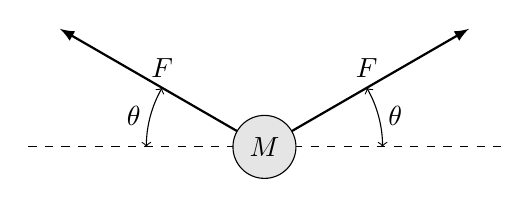
\begin{tikzpicture}
        %% Forces
        \draw[thick,-latex] (0,0) -- (30:3) node[pos=0.5,anchor=south] {$F$};
        \draw[thick,-latex] (0,0) -- (150:3) node[pos=0.5,anchor=south] {$F$};
        %% angle
        \draw[dashed] (-3,0) -- (+3,0);
        \draw[<->] (+1.5,0) arc (0:30:1.5) node[pos=0.5,anchor=west] {$\theta$};
        \draw[<->] (-1.5,0) arc (180:150:1.5) node[pos=0.5,anchor=east] {$\theta$};
        %% Ball
        \node[draw,circle,minimum size=0.8cm,fill=white!90!black,anchor=center] at (0,0) {$M$};
    \end{tikzpicture}
    \end{center}
    The angle $\theta$ that the rope makes with the horizontal is,
    \begin{choices}
        \wrongchoice{\ang{56}}
        \wrongchoice{\ang{5.6}}
      \correctchoice{\ang{0.56}}
        \wrongchoice{\ang{0}; the rope will obviously be horizontal in this situation.}
    \end{choices}
\end{question}
}


%% CAP Exam 1994 Part A: Multiple Choice Questions
%%--------------------------------------------------
\element{cap}{
\begin{question}{CAP-A-1994-q01}
    It was once proposed to use a \SI{2}{\kilo\meter} vertical Sudbury mine shaft for microgravity experiments in a vacuum.
    How much time would scientists have to do an experiment during one drop?
    \begin{multicols}{2}
    \begin{choices}
      \correctchoice{\SI{20}{\second}}
        \wrongchoice{\SI{63}{\second}}
        \wrongchoice{\SI{0.64}{\second}}
        \wrongchoice{\SI{198}{\second}}
    \end{choices}
    \end{multicols}
\end{question}
}

\element{cap}{
\begin{question}{CAP-A-1994-q02}
    If the moon were twice as massive as it is now,
        and it stayed at the same orbital radius about the earth as it has now,
        its new orbital period (in terms of its current orbital period $T$) would be:
    \begin{multicols}{4}
    \begin{choices}
      \correctchoice{$T$}
        \wrongchoice{$\dfrac{T}{2}$}
        \wrongchoice{$\dfrac{T}{4}$}
        \wrongchoice{$2T$}
    \end{choices}
    \end{multicols}
\end{question}
}

\element{cap}{
\begin{question}{CAP-A-1994-q03}
    In the following circuit composed of identical capacitors,
    \begin{center}
    \begin{circuitikz}
        %% NOTE: TODO: draw
    \end{circuitikz}
    \end{center}
        across which terminals would you connect a battery in order for all the capacitors to charge up.
    \begin{multicols}{2}
    \begin{choices}
        \wrongchoice{$AB$}
        \wrongchoice{$AC$}
      \correctchoice{$BD$}
        \wrongchoice{none of the provided}
    \end{choices}
    \end{multicols}
\end{question}
}

\element{cap}{
\begin{question}{CAP-A-1994-q04}
    Two cylindrical resistors, one of length $l$ and radius $r$,
        and the other of length $3l$ and radius $3r$,
        are made of the same materials.
    If the resistance of the smaller one is $R$,
        what is the resistance of the larger one?
    %% R = \rho l / A
    \begin{multicols}{4}
    \begin{choices}
      \correctchoice{$\dfrac{R}{3}$}
        \wrongchoice{$3 R$}
        \wrongchoice{$9 R$}
        \wrongchoice{$27 R$}
    \end{choices}
    \end{multicols}
\end{question}
}

\element{cap}{
\begin{question}{CAP-A-1994-q05}
    A simple pendulum consists of a mass $m$ attached to a light string of length $l$.
    If the system is oscillating through small angles,
        which of the following is true?
    \begin{choices}
        \wrongchoice{The frequency is independent of the acceleration due to gravity $g$.}
        \wrongchoice{The period depends on the amplitude of the oscillation.}
      \correctchoice{The period is independent of the mass $m$.}
        \wrongchoice{The period is independent of the length $l$.}
    \end{choices}
\end{question}
}

\element{cap}{
\begin{question}{CAP-A-1994-q06}
    An astronaut in the space shuttle orbiting the earth performs a trick for a television audience.
    She inflates a helium filled balloon within the shuttle's controlled atmosphere and lets go of it.
    To the astonishment of all watching, the balloon:
    \begin{choices}
      \correctchoice{hoovers in place where it was released.}
        \wrongchoice{rises noticeably away from the earth.}
        \wrongchoice{falls noticeably towards the earth.}
        \wrongchoice{drifts backwards opposite to the direction of the shuttle's velocity}
    \end{choices}
\end{question}
}

\element{cap}{
\begin{question}{CAP-A-1994-q07}
    A boat has a green light (with wavelength $\lambda=\SI{500}{\nano\meter}$) on its mast.
    What wavelength would be measured and what color would be observed for this light as seen by a diver submerged in water (index of refraction $n=1.33$) by the side of the boat.
    \begin{choices}
        \wrongchoice{Green $\lambda=\SI{500}{\nano\meter}$}
        \wrongchoice{Red $\lambda=\SI{665}{\nano\meter}$}
      \correctchoice{green $\lambda=\SI{376}{\nano\meter}$}
        \wrongchoice{UV $\lambda=\SI{376}{\nano\meter}$}
    \end{choices}
\end{question}
}

\element{cap}{
\begin{question}{CAP-A-1994-q08}
    A radio station transmits using a vertical mast.
    The antenna in your radio is a coil (solenoid) wrapped around a ferrite (iron) rod.
    What orientation must this antenna have for optimum reception?
    \begin{choices}
        \wrongchoice{Rod pointing at mast.}
        \wrongchoice{Rod parallel at mast.}
      \correctchoice{Horizontal rod pointing \ang{90} from the line of the mast.}
        \wrongchoice{Horizontally oriented rod directly above the mast.}
    \end{choices}
\end{question}
}

\element{cap}{
\begin{question}{CAP-A-1994-q09}
    You have ten identical filters.
    One is placed in front of a white light and the light appears red.
    When all ten are placed in front of the light,
        it appears to be a dim green color.
    Which of the following is a possible transmission characteristic for one of the filters?
    \begin{multicols}{2}
    \begin{choices}
        %% NOTE: TODO: draw tikz graph
        %% NOTE: ANS is A
        \wrongchoice{
            \begin{tikzpicture}
            \end{tikzpicture}
        }
    \end{choices}
    \end{multicols}
\end{question}
}

\element{cap}{
\begin{question}{CAP-A-1994-q10}
    Two atoms interact with each other according to the following force $F$,
        and potential, $V$ diagrams.
    What is their equilibrium separation?
    \begin{center}
    \begin{tikzpicture}
        %% NOTE: TODO: draw pgfplots
    \end{tikzpicture}
    \end{center}
    \begin{choices}
        \wrongchoice{The separation $u$ which is equal to $y$}
      \correctchoice{The separation $u$ which is equal to $z$}
        \wrongchoice{The separation $w$ which is equal to $y$}
        \wrongchoice{The separation $w$ which is equal to $z$}
    \end{choices}
\end{question}
}

\element{cap}{
\begin{question}{CAP-A-1994-q11}
    A ball is thrown into the air with an initial speed $u$.
    The time interval taken for the ball to rise to its maximum height is $t_r$.
    The time interval taken for it to fall back down from this maximum height to its original position is $t_f$.
    Under ``real life'' conditions,
        which of the following is satisfied by $t_r$ and $t_f$?
    \begin{choices}
        \wrongchoice{$t_r > t_f$}
      \correctchoice{$t_r < t_f$}
        \wrongchoice{$t_r = t_f$}
        \wrongchoice{$t_r > t_f$ if $u$ is great enough.}
    \end{choices}
\end{question}
}

\element{cap}{
\begin{question}{CAP-A-1994-q12}
    An airplane flied a straight path from town $A$ to town $B$, \SI{5 000}{\kilo\meter} away.
    Town $B$ is due east of town $A$ and a strong wind blow from north to south at \SI{300}{\kilo\meter\per\hour}.
    If the plane's airspeed is \SI{900}{\kilo\meter\per\hour},
        which of the following statements is true?
    \begin{choices}
      \correctchoice{Trip time is $\dfrac{5}{3\sqrt{8}}\,\si{\hour}$} 
        \wrongchoice{Plane's ground speed is \SI{600}{\kilo\meter\per\hour}.}
        \wrongchoice{Plane's heading is \ang{30} North of East.}
        \wrongchoice{None of the provided.}
    \end{choices}
\end{question}
}

\element{cap}{
\begin{question}{CAP-A-1994-q13}
    Microwaves of wavelength $\lambda=\SI{5.0}{\centi\meter}$,
        and intensity $I_0$ are split and recombined by the metallic mirror system shown.
    \begin{center}
    \begin{tikzpicture}
        %% NOTE: TODO: draw tikz
    \end{tikzpicture}
    \end{center}
    What should $x$ be so that the intensity of the microwaves at the point $P$ (the detector) is zero?
    \begin{multicols}{2}
    \begin{choices}
        \wrongchoice{\SI{0.88}{\centi\meter}} 
        \wrongchoice{\SI{3.54}{\centi\meter}} 
      \correctchoice{\SI{6.04}{\centi\meter}} 
        \wrongchoice{\SI{3.02}{\centi\meter}} 
    \end{choices}
    \end{multicols}
\end{question}
}

\element{cap}{
\begin{question}{CAP-A-1994-q14}
    Which of the following is a possible expression for the Rydberg, a unit of energy?
    \begin{multicols}{2}
    \begin{choices}
        \wrongchoice{$\dfrac{e^4}{8m_e \epsilon_0 h^2}$}
        \wrongchoice{$\dfrac{\epsilon_0^2 h^2}{8m_e e^4}$}
      \correctchoice{$\dfrac{m_e e^4}{8 \epsilon_0^2 h^2}$}
        \wrongchoice{$\dfrac{m_e c^2}{\epsilon_0 h e}$}
    \end{choices}
    \end{multicols}
\end{question}
}

\element{cap}{
\begin{question}{CAP-A-1994-q15}
    Consider the network of identical resistors shown.
    \begin{center}
    \begin{tikzpicture}
        %% NOTE: TODO: circuitikz
    \end{tikzpicture}
    \end{center}
    The equivalent resistance between the points $A$ and $B$ is:
    \begin{multicols}{2}
    \begin{choices}
        \wrongchoice{$5R$}
        \wrongchoice{$\dfrac{R}{2}$}
      \correctchoice{$\dfrac{5R}{8}$}
        \wrongchoice{$2R$}
    \end{choices}
    \end{multicols}
\end{question}
}

\element{cap}{
\begin{question}{CAP-A-1994-q16}
    A ray of light is directed towards a corner reflector as shown.
    The incident ray makes an angle of \ang{22} with one of the mirrors.
    \begin{center}
    \begin{tikzpicture}
        %% NOTE: TODO: circuitikz
    \end{tikzpicture}
    \end{center}
    At what angle $\theta$ does the ray emerge?
    \begin{multicols}{2}
    \begin{choices}
        \wrongchoice{\ang{22}}
      \correctchoice{\ang{68}}
        \wrongchoice{\ang{44}}
        \wrongchoice{none of the provided}
    \end{choices}
    \end{multicols}
\end{question}
}

\element{cap}{
\begin{question}{CAP-A-1994-q17}
    Many people's glasses appear to be a glue-green color when viewed under reflected light.
    A thin film of index of refraction $n=1.35$ is applied to the outside surface of the glass so that the film/glass interface does not reflect any red light of wavelength $\lambda=\SI{630}{\nano\meter}$.
    What thickness must the film layer be in order to achieve this?
    Take the index of refraction of air and glass to be 1.0 and 1.6 respectively.
    \begin{multicols}{2}
    \begin{choices}
        \wrongchoice{\SI{157.5}{\nano\meter}}
        \wrongchoice{\SI{315.0}{\nano\meter}}
        \wrongchoice{\SI{233.3}{\nano\meter}}
      \correctchoice{\SI{116.7}{\nano\meter}}
    \end{choices}
    \end{multicols}
\end{question}
}

\element{cap}{
\begin{question}{CAP-A-1994-q18}
    A mass $M$ has the same kinetic energy as a mass $m$.
    The ratio of their momentum, $p_M / p_m$, is:
    \begin{multicols}{2}
    \begin{choices}
      \correctchoice{$\sqrt{\dfrac{M}{m}}$}
        \wrongchoice{$\sqrt{\dfrac{m}{M}}$}
        \wrongchoice{$\dfrac{m+M}{M}$}
        \wrongchoice{$\dfrac{\left(m+M\right)^2}{mM}$}
    \end{choices}
    \end{multicols}
\end{question}
}

\element{cap}{
\begin{question}{CAP-A-1994-q19}
    A stream of water droplets, each of mass $m=\SI{0.001}{\kilo\gram}$,
        are fired horizontally at a velocity of \SI{10}{\meter\per\second} towards a steel plate where they collide.
    The droplets are spaced equidistantly with a spacing of \SI{1}{\centi\meter}.
    What is the approximate average force exerted on the plate by the water droplets assuming that they do not rebound after their collision.
    \begin{multicols}{2}
    \begin{choices}
      \correctchoice{\SI{10}{\newton}}
        \wrongchoice{\SI{100}{\newton}}
        \wrongchoice{\SI{1}{\newton}}
        \wrongchoice{\SI{0.1}{\newton}}
    \end{choices}
    \end{multicols}
\end{question}
}

\element{cap}{
\begin{question}{CAP-A-1994-q20}
    Three identical balls are thrown from the top of a cliff and some time later land at the base of the cliff.
    Ball $A$ is thrown upwards with speed $v$, Ball $B$ is thrown downwards with speed $v$,
        and Ball $C$ is thrown at speed $v$ and at an angle of \ang{45} above the horizontal.
    Comparing the speeds, $v_A$, $v_B$, and $v_C$ with which the balls hit the ground at the base of the cliff (and ignoring air resistance), you find:
    \begin{multicols}{2}
    \begin{choices}
        \wrongchoice{$v_A = v_B > v_C$}
        \wrongchoice{$v_A > v_C > v_B$}
      \correctchoice{$v_A = v_B = v_C$}
        \wrongchoice{$v_B > v_C > v_A$}
    \end{choices}
    \end{multicols}
\end{question}
}


\endinput


